\documentclass{book}
\usepackage[utf8]{inputenc}
\usepackage{ bussproofs }
\usepackage{ amssymb }
\usepackage{hyperref}
\usepackage{listings}
\usepackage{xargs}
\usepackage{simplebnf}
\usepackage{float}
\usepackage{xcolor}
\usepackage{numprint}
\usepackage{ amsmath }
\usepackage{mathpartir}
\usepackage{minted}
\usemintedstyle{colorful}
\usepackage[hashEnumerators,smartEllipses, hybrid]{markdown}
\usepackage{amsthm}
\usepackage{csquotes}
\usepackage{ stmaryrd }
\usepackage{stackengine,scalerel}
\usepackage[british]{babel}

\usepackage[bibstyle=numeric, backend=bibtex]{biblatex}
\addbibresource{../Meine Bibliothek.bib}

% % dark mode
% \usemintedstyle{monokai}
% \usepackage{draculatheme}



\usepackage[colorinlistoftodos,prependcaption,textsize=tiny]{todonotes}

\newcommandx{\unsure}[2][1=]{\todo[linecolor=red,backgroundcolor=red!25,bordercolor=red,#1]{#2}}
\newcommandx{\change}[2][1=]{\todo[linecolor=blue,backgroundcolor=blue!25,bordercolor=blue,#1]{#2}}
\newcommandx{\info}[2][1=]{\todo[linecolor=OliveGreen,backgroundcolor=OliveGreen!25,bordercolor=OliveGreen,#1]{#2}}
\newcommandx{\improvement}[2][1=]{\todo[linecolor=Plum,backgroundcolor=Plum!25,bordercolor=Plum,#1]{#2}}
\newcommand{\code}[1]{\texttt{#1}}

\newcommand{\mtext}[1]{$\text{#1}$}
\newcommand{\tuple}[2]{\langle #1 \mid #2 \rangle}
\newcommand{\bbracket}[1]{\llbracket #1 \rrbracket}

\DeclareMathOperator{\rref}{ref}



\newcommand{\ccolon}[0]{: }
\newcommand{\cmid}[0]{| }
\newcommand{\cdisj}[0]{|| }


\newtheorem{theorem}{Theorem}[section]
\newtheorem{corollary}{Corollary}[theorem]
\newtheorem{lemma}[theorem]{Lemma}
\theoremstyle{definition}
\newtheorem{definition}[theorem]{Definition}

\begin{document}

\tableofcontents


Software correctness is a central goal for software development.
One way to improve correctness is using strong and descriptive types and verifying them with type systems.
In particular Refinement Types demonstrated, that even with a verification system that is restricted to a decidable logic, intricate properties can be expressed and verified in a lightweight and gradual way.
However existing approaches for adapting Refinement Types from functional to imperative languages proved hard without compromising on at least one of core features of Refinement Types.
% I argue that a base language restricted to unique mutable references will make
This thesis aims to design a Refinement Type system without such compromises by taking advantage of Rust's restriction to unique mutable references.
I will define a Refinement Type language and typing rules and argue for their soundness. Additionally I will implement a prototype verifier to evaluate the effectiveness of the approach on selected examples.





\chapter{Introduction}

% With increasing reliance on increasingly complex software, ensuring correctness of programs is a vital concern to software development.
With increasing amount and reliance of software, ensuring the correctness of programs is a vital concern for the future of software development.
Although research in this area has made good progress, most approaches are not accessible enough for general adoption by the developers. Especially in light of a predicted shortage of developers\cite{breaux_2021_2021-1}, it is not sufficient to require developers to undergo year-long training in specialized and complex verification methods to ensure the correctness of their software. It is therefore crucial to integrate with their existing tooling and workflows to ensure the future high quality of software.
One avenue for improving accessability for functional verification is extending the expressiveness of the type system to cover more of the correctness properties.
Using type systems for correctness was traditionally prevalent in purely functional languages where evolving states are often represented by evolving types, offering approachable and gradual adoption of verification methods. Tracing evolving states in the type system would be especially useful for languages with mutability, since substantial parts of the behaviour of the program is expressed as mutation of state. In particular Rust seems like a promising target language, because mutability is already tracked precisely and thus promising functional verification for relatively minimal effort on the programmer's part.

The goal of the thesis is to show that Refinement Types can be idiomatically adapted to languages with unique mutable references. The type system presented in this thesis enables gradual adoption of lightweight verification methods in mutable languages.

%In case implementing these translations could not be completed, the use cases will be transformed manually.
The type system is sound and effective in the identified use-cases.
%In addition, a description of the syntax and semantics of the constructs, that will extend Rust's type system, will be provided as well as justification for their soundness. 
A feasibility study on minimal examples of challenging use cases shows how useful the proposed verification system is. 
%For use cases that could not be covered by the proposed additions, the reason will be investigated.

Specifying or verifying complete Rust modules or the entire Rust language is not the goal of the thesis. In particular \code{unsafe} Rust will not be taken into account in specification nor implementation. Implementing Liquid Type inference in also not a goal of the thesis.

The accompanying implementation extends the Rust compiler, enables automatic parsing of the refinement type language and automated type checking of a subset of Rust, as well as limited inference and error reporting. 
The thesis also gives a description of the syntax and semantics of the subset of Rust as well as the refinement type system.

The contributions of this thesis are:
\begin{enumerate}
  \item Automatic empirical analysis of the usage of mutability and unsafe in Rust using syntactic information
  \item Extension to the Rust type system to allow for refinement type specifications
  \item Description and implementation of a type checker for the introduced type system
  \item Evaluation of the type system on minimal benchmarks
\end{enumerate}

The thesis if structured as follows: 
In chapter XXX an empirical analysis of \code{unsafe} and mutability uses is performed. 
Then chapter XXX will give an overview of the foundation the thesis build upon. 
Chapter XXX defines the subset of Rust, that will be the basis for the type system.
Next chapter XXX explains the actual type system and verification, as well as justifying its correctness, followed by chapter XXX, which will provide more information about the implementation.
The type system will then be tested in minimal benchmarks in chapter XXX.
Chapter XXX reports on related work and alternative approaches.
Finally chapter XXX concludes the thesis and gives an overview over possible future work.


\chapter{Empirical Analysis of Use-Cases}

Before designing a system for Rust, it makes sense to gain some understanding of how Rust is used. For this purpose we will look at two key features of Rust, that influence how an approachable verification should look like.
Firstly \code{unsafe} Rust with similar guarantees to C would make verification and specification significantly harder. But if the use of \code{unsafe} is limited, like intended by the language designers, it would allow us to focus on the save part of Rust and leave the verification of \code{unsafe} Rust to more complex verification systems.
Secondly with mutability being the main difference to the traditional domain fof Refinement Types, showing the need for covering this area and to what degree of approachability it interesting.

There are two fundamental questions, that analysing existing rust code should answer: 
\begin{enumerate}
  \item \label{enum:hypothesis-unsafe-rare} How rare are uses of \code{unsafe}
  \item \label{enum:hypothesis-unsafe-lib} How much effort is acceptable when specifying \code{unsafe} code?
  \item \label{enum:hypothesis-mut} How common are mutable variables and references in Rust?
\end{enumerate}

To check these assumptions an analysis of existing Rust code was performed. As a basis for the analysis, the Rust package registry \href{https://www.crates.io}{crates.io} was used. It contains the source code for both Rust libraries as well as various applications written in Rust (e.g. ripgrep). 

We analyzed all published Rust crates (Rust's version packages) on February 2nd 2022 on crates.io with at least 10 versions\footnote{The limit of 10 versions is used to eliminate inactive and placeholder packages}, which totals \numprint{11882} crates, containing \numprint{228263} files with a combined code-base size of over 64 million lines of Rust code (without comments and white space lines)\footnote{Calculated with \texttt{cloc}}. 

% from cloc
% ----------------------------------------------------------------------------------------
% Language                              files          blank        comment           code
% ----------------------------------------------------------------------------------------
% Rust                                 228263        5664979       10317162       64193670
% C                                     32945        1539542        1979846       13468919
% C++                                   18084        1263696        1093652        7956897
% JSON                                  15838           1897              0        6424252
% C/C++ Header                          31619        1152322        2015896        6284146
% XML                                    5142          25277          25773        4807556
% Assembly                               4146         534785         582345        2631991

The analysis parses these files and searches for certain AST patterns, which are subsequently extracted and saved.
Thanks to using the tree-sitter parsing framework, the analysis framework can easily be extended to other queries and languages.

\label{ss:unsafe-rust}\section{Unsafe Rust}

Firstly we will be answering the question of \code{unsafe} usage in Rust.
There is already some research on how \code{unsafe} is used in Rust. For example Astrauskas et al. \cite{astrauskas_how_2020} found, that about 76\% of crates did not use any unsafe. On top of that, unsafe signatures are only exposed by 34.7\% of crates, that use \code{unsafe}.

"The majority of crates (76.4\%) contain no unsafe features at all. Even in most crates that do contain unsafe blocks or functions, only a small fraction of the code is unsafe: for 92.3\% of all crates, the unsafe statement ratio is at most 10\%, i.e., up to 10\% of the codebase consists of unsafe blocks and unsafe functions." \cite[p. 13]{astrauskas_how_2020}
Our data seems to confirm this: \numprint{8044} of the \numprint{11882} crates (67.7\%) did not use any unsafe. 

Astrauskas et al. also found, that "however, with 21.3\% of crates containing some unsafe statements and – out of those crates – 24.6\% having an unsafe statement ratio of at least 20\%, we cannot claim that developers use unsafe Rust sparingly, i.e., they do not always follow the first principle of the Rust hypothesis." \cite[p. 14]{astrauskas_how_2020}

When checking unsafely for our use case, it makes sense to further distinguish between libraries and executables crates: Libraries are intended to be used by other Rust programs: Usage of unsafe in libraries may not be as problematic as in executables, because libraries are written once but used by many applications, justifying higher verification effort. 

In our analysis we found, that firstly crates.io contains significantly more libraries than binaries\footnote{Libraries and Executables are distinguished by checking if they contain \code{bin} or \code{lib} target or one of the corresponding files according to the cargo naming convention.} (see Figure \ref{fig:crate_types}). 
And secondly libraries are much more likely to use \code{unsafe} Rust. Table shows the result of our analysis. Where uses of \code{unsafe} are counted and grouped by crate type (see Table \ref{tab:unsafe-uses-by-crate}).
The data in the table includes all crates except the outlier \code{windows-0.32.0}, which alone contains \numprint{233608} uses of \code{unsafe}. Nearly $2 / 3$ of all other library uses of \code{unsafe} combined.
Looking at the distribution of unsafe uses in Figure \ref{fig:unsafe-hist}, we can see, that this is an exception: Most other libraries do not use that much unsafe statements. We can also see, that even if a executable crate uses \code{unsafe}, it uses few.



\begin{figure}[h]
	\centering
	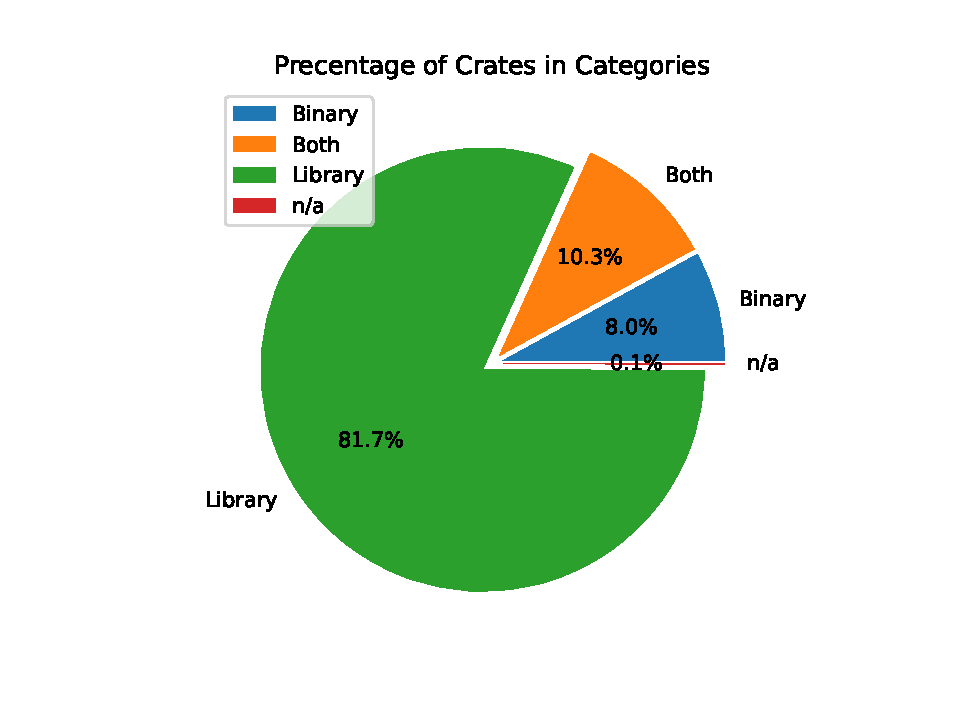
\includegraphics[width=0.7\linewidth, clip, trim={0.5cm 0.5cm 0.5cm 0.5cm}]{../crate_types.pdf}
	\caption{Percentage of Crates, that Contain Libraries, Executables or Both}
	\label{fig:crate_types}
\end{figure}

\begin{table}[h]
\centering
\begin{tabular}{l | r}
  & Number of Unsafe Uses \\
  Crate Type &  \\
  \hline
 Library & \numprint{382997} \\
 Both & \numprint{7720} \\
 Binary & \numprint{930} \\
 n/a & \numprint{215} \\
 \end{tabular}
\caption{Number of Unsafe Uses by Crate Category}
\label{tab:unsafe-uses-by-crate}
\end{table}



\begin{figure}[h]
	\centering
	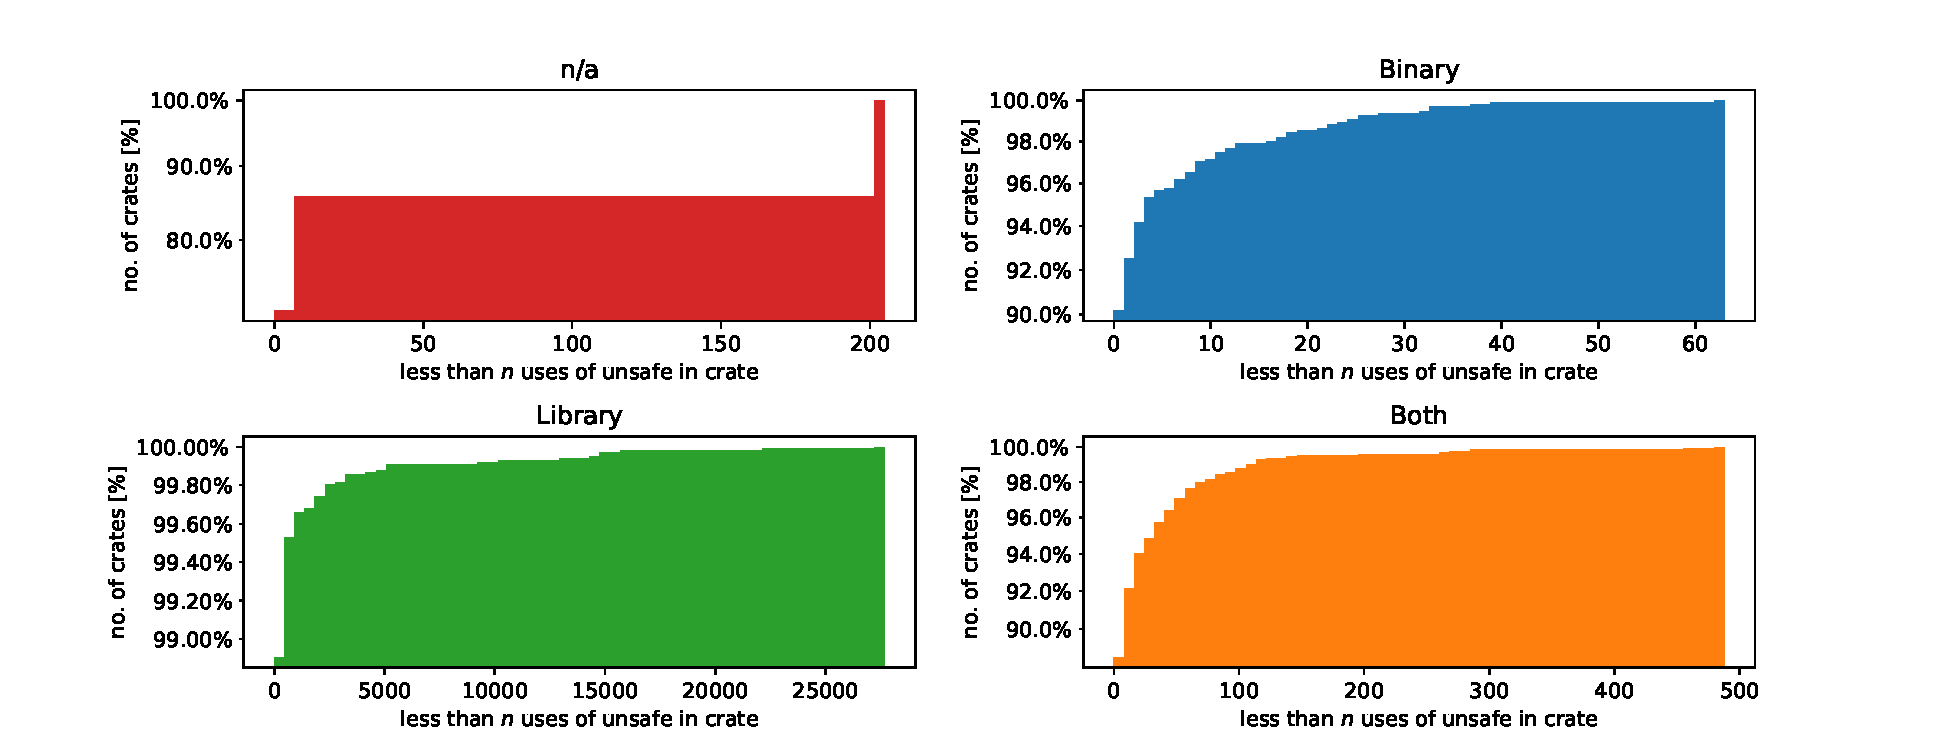
\includegraphics[width=0.99\linewidth, clip, trim={0.2cm 0.2cm 0.2cm 0.2cm}]{../unsafe_counts_by_crate_type.pdf}
	\caption{Cumulative, logarithmic histogram of the amount of \code{unsafe} uses in each category}
	\label{fig:unsafe-hist}
\end{figure}


\section{Mutability}

Finally we will analyse how common mutable variables and references are used in Rust. 
The frequency of usage will inform the acceptable level of specification effort.

To analyse the dataset for usage pattern, we search the dataset for certain syntactical structures to infer mutability information about the following various AST items:
\begin{itemize}
	\item \textbf{Local Variable Definitions} can be tracked with high confidence. They occur in function bodies and take the form: \code{let mut a = <expr>}
	\item \textbf{Parameters}, which are considered immutable if they are passed as immutable references or owned. They take the syntactic form: \code{mut a: i32} or \code{b: \&mut i32}
	\item \textbf{Function Definitions}, which are considered immutable, if all parameters considered immutable. They take the syntactic form: \code{fn f(mut a: i32, b: \&mut i32) \{ ... \}}
	\item \textbf{Arguments} are parts of a function call and can be arbitrary expression, which makes the tracking hard.
	\item \textbf{Function Calls}, which are considered immutable, if all arguments are considered immutable.
\end{itemize}

A total of around 52 million of these items were found in the dataset.

Figure~\ref{fig:mutabillity_by_category} shows the ratio of mutable to immutable items. For each syntactical category, the percentages are given relative to different objects:

\begin{enumerate}
  \item Total: number of occurrences
  \item Function: number of unique functions. I.e. 76.54\% of functions have a immutable parameter.
  \item File: number of unique files
\end{enumerate}


\begin{figure}[h]
	\centering
	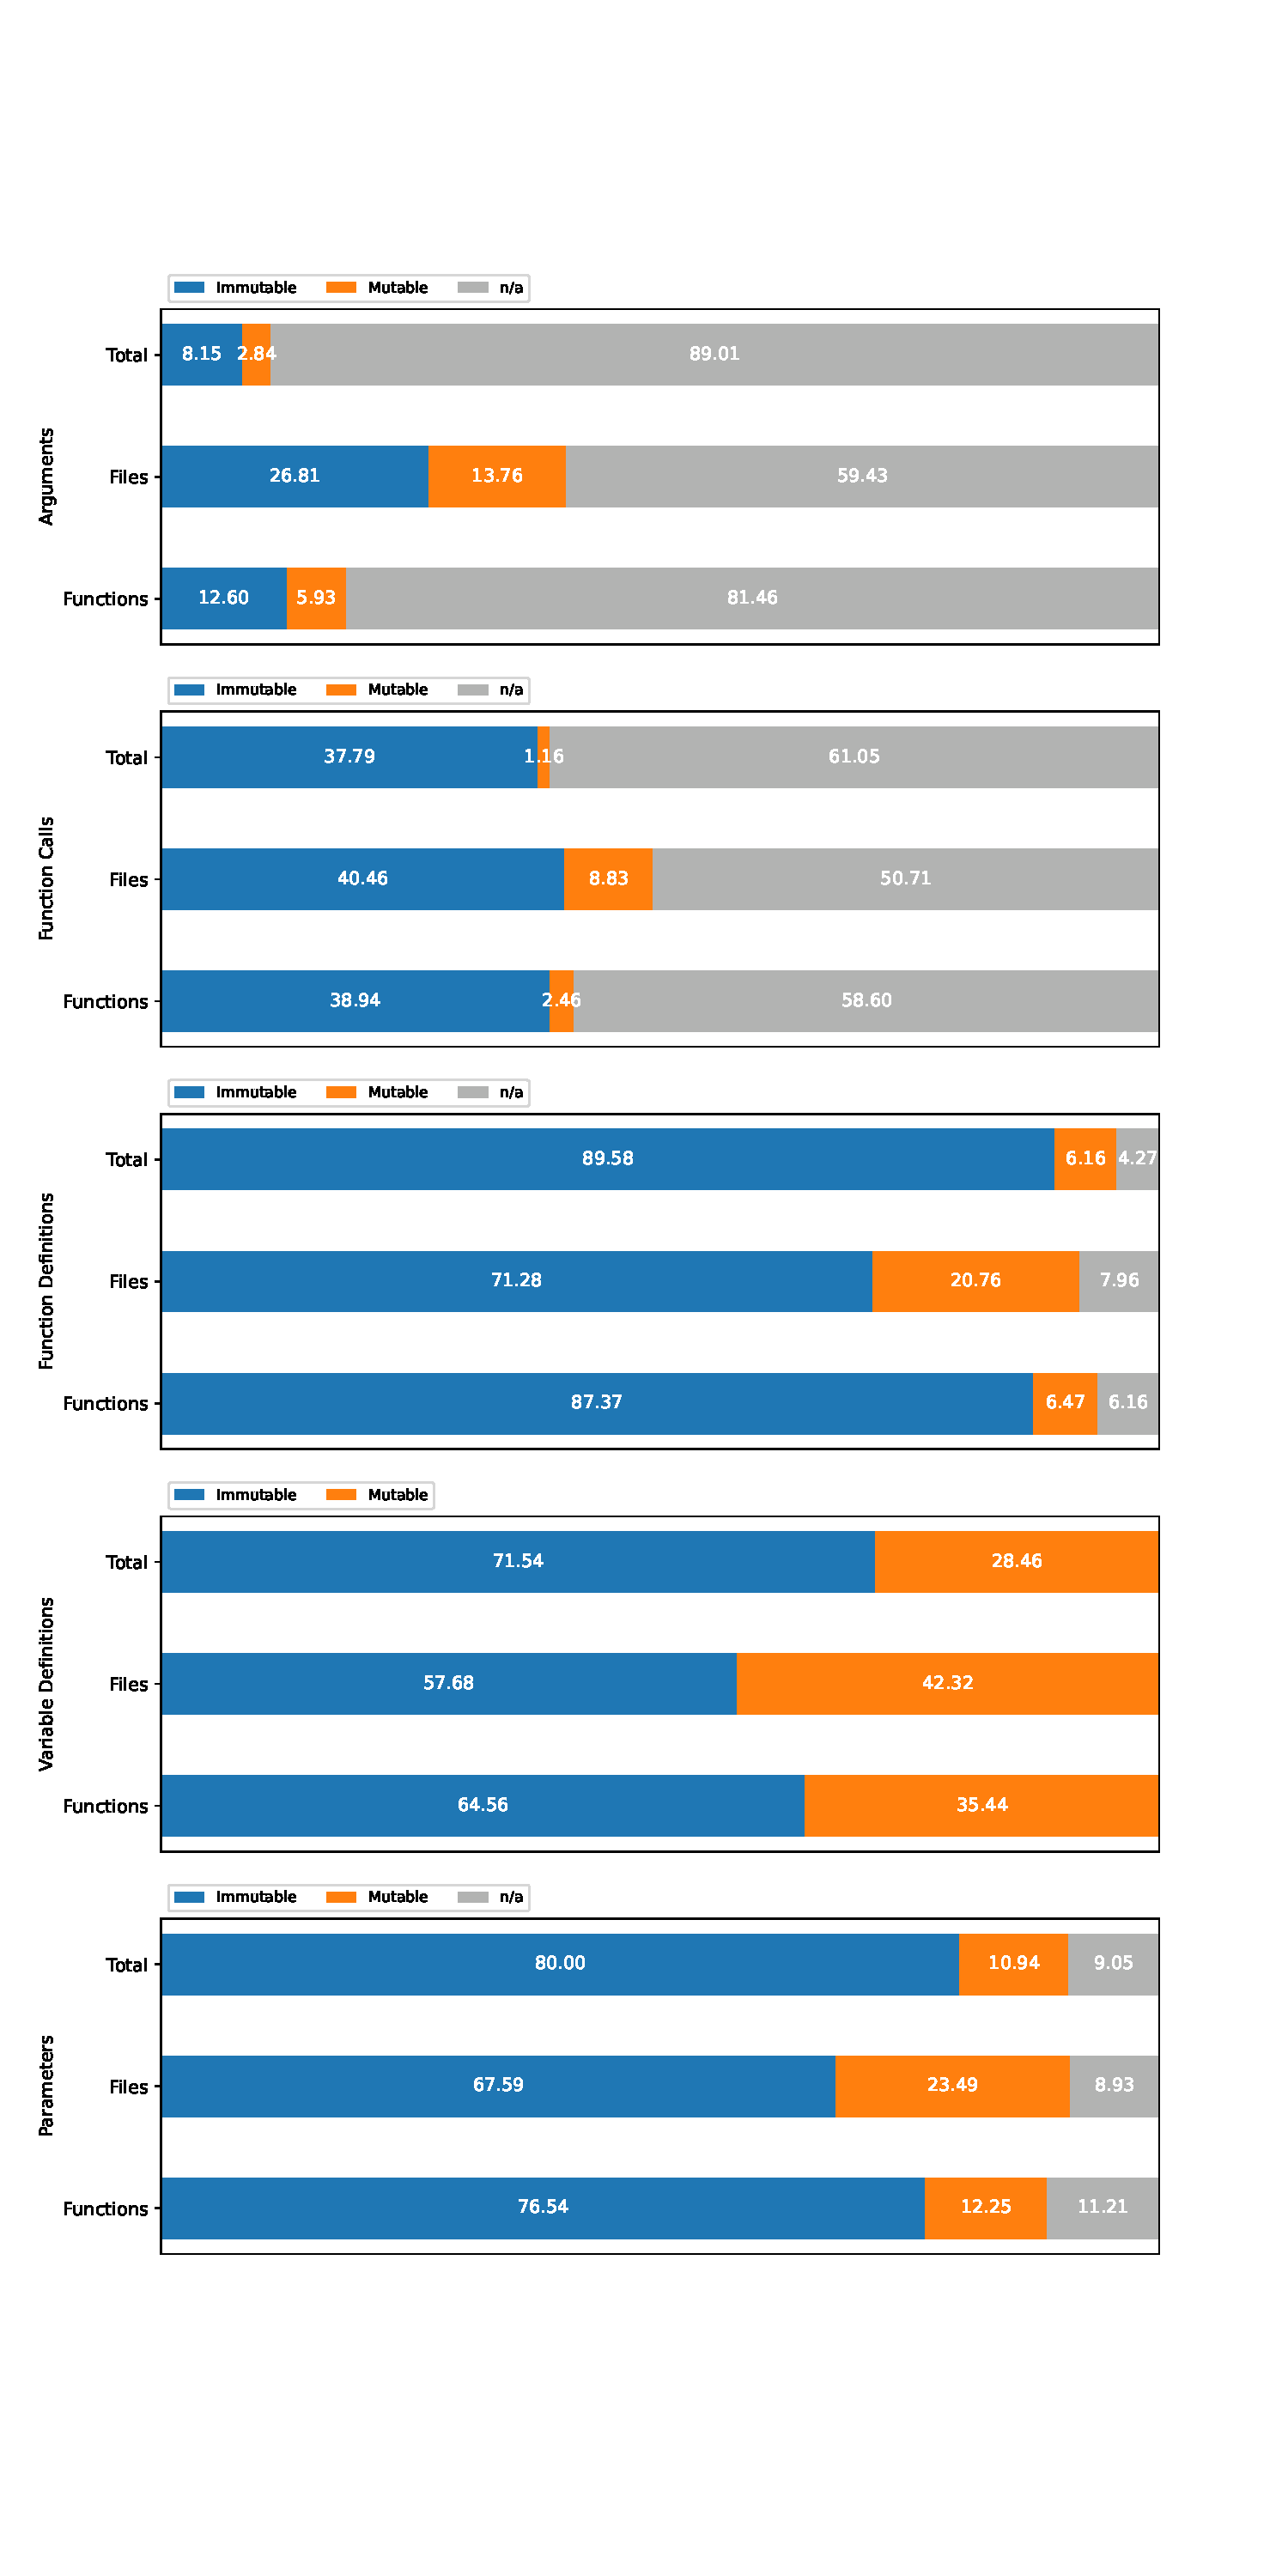
\includegraphics[width=0.9\linewidth, clip, trim={0.5cm 6cm 0.5cm 6cm}]{../mutability_by_category.pdf}
	\caption{Ratio of Immutable to Mutable Versions of Different AST Items. Items are Counted by Unique Occurrences}
	\label{fig:mutabillity_by_category}
\end{figure}

Unfortunately not there are some areas, where the syntactic analysis is not sufficient. Namely the analysis of function calls and arguments, which is mainly caused by the uncertainty of mutability of complex arguments.
Luckily the data from function definitions and parameters can complete the picture: About 80\% of parameters are immutable and between about 10 and 20\% of parameters are mutable. And less than 10\% of functions have mutable parameters at all.
When it comes to local variables, Rust users are more liberal in their use of mutability:
About 30\% of local variables are defined mutable.

For verification this means, that the use of mutability is wide spread. Especially local variables are often mutable and should therefore a verification system should try to minimize the effort for the user. Mutable parameters are less common, but still need to be accounted for in verification.

\section{Conclusions}

For this thesis the following conclusion can be drawn:

\begin{itemize}
  \item Even though uses of \code{unsafe} are not rare, it is acceptable to ignore in favour of a simpler type system.
  \item Mutable variables are used very often and should therefore have very little associated specification effort.
  \item Mutable parameters are used less frequently justifying a higher specification effort, but their specification must still be possible.
\end{itemize}

\chapter{Foundations}

This chapter will introduce 


\section{Refinement Types}

The type system, that this thesis will adapt, is based on the Refinement Type system described by Vazou et al. \cite{vazou_abstract_2013} and Rondon et al. \cite{rondon_liquid_2008}. 
The central idea of Refinement Types is adding predicates to a language's type: For example, a type \code{i32} might be refined with the predicate $v > 0$. The refined type is written as $\left\{ v : \text{i32} \mid v > 0 \right\}$. In terms of semantics this means, that any inhabitant of that type must also satisfy the predicate. 

The notion of refinements in embedded into the base language using subtyping: A refined type $\tau$ is a subtype of $\tau'$ if $\tau$'s predicate implies the predicate of $\tau'$ (in the current typing context $\Gamma$).
As is common with subtyping systems, the subtype can then be used in the place where the super type is expected.
The following rule shows how subtyping is handled by Liquid types \cite[p. 6]{rondon_liquid_2008}:

\begin{equation*}
  \inferrule*
    {\text{SMT-Valid}(\llbracket \Gamma \rrbracket \wedge \llbracket e_1 \rrbracket \Rightarrow \llbracket e_2 \rrbracket)}
    {\Gamma \vdash \left\{ v : b \mid e_1 \right\} \preceq \left\{ v: b \mid e_2 \right\}}
\end{equation*}

Refinement Types are related to dependent types, distinguished by the limited expressiveness of the type. Refinement types trade off expressiveness for automatic type checking. Allowed formulas are chosen from a SMT decidable logic. 
Rondon et al. \cite{rondon_liquid_2008} chose the EUFA as the logic fragment, meaning a propositionaly logic with the theories of equality, uninterpreted functions and linear arithmetic.


\section{Rust}

The Rust programming language, first conceived of by Graydon Hoare, is multi-paradigm programming language, that draws inspiration from functional and imperative programming languages. The core forms a set of features usually found in functional programming languages: Functions, closures, algebraic data types, type classes (called traits in Rust) and pattern matching, immutability are all common place in Rust.
But what is unusual is, that Rust extends this base with optional mutability of data and references. The Rust programming language is design to closed control the amount of mutability and what it can effect. To this end, Rust incorporates the notion of affine types into its type system (called ownership system in Rust).
Rust took inspiration from a research language called Cyclone introduced by Grossman et al. \cite{grossman_region-based_nodate}.
Among other things, the ownership system is used to handle memory management, safe concurrency and simplifies reasoning about program behaviour.
The next paragraph will explain how the ownership system works.

\paragraph{Aliasing XOR Mutabillity} The key behind Rusts ownership system is, that for every variable at every point during the execution, that variable can either aliased or mutable, but never both at the same time.

Rust accomplished this by introducing three types of access permissions for a variable, which are associated with every scope\footnote{In modern Rust, this model was generalized to cover more cases, but the idea is still valid}:
\begin{enumerate}
  \item The scope \textit{owns} the variable. This guarantees, that no other scope has access to any part of the variable and allows the scope to create references to (part of) the variable.
  \item The scope (immutably) \textit{borrows} the variable. This guarantees, that as long as the variable is used, its \textit{value will not change} and allows the scope to further lend the variable to other scoped.
  \item The scope \textit{mutably borrows} the variable. This guarantees, that there are no other active references to any part of the memory of the variable.
\end{enumerate}

A consequence of these rules it, that at any time, every piece of memory has a unique and compile-time known owner. There are no reference cycles.

This makes both aliasing as well as mutability quite tame:
If a variable is aliased, it must be immutable and as a result, represents just a value (like in pure functional languages).
If a variable is mutable, it can not be aliased and as a result, any effect of the mutation is well known and locally visible.

\subsection{The Case for Rust as a Target Language}


Rust justifies a new approach to mutable verification, because it is possible to take advantage of guarantees provided by (safe) Rust's ownership system. 

Rust is split into two languages: safe and unsafe Rust. Like most type systems, Rust's type and ownership system is conservative, meaning any (safe) Rust program that type checks, will not crash due to memory safety or type errors. Unsafe Rust gives the programmer the ability to expand the programs accepted by Rust outside that known-safe subset.

In this thesis, we will only consider safe Rust, which is the subset of Rust most programmers interact with (see section \ref{ss:unsafe-rust}).

Rust features a few unusual design decisions that profoundly influence the design of verification systems for it. The following paragraphs will elaborate on this.


\paragraph*{Opaque Generics} Rust does not provide a way to check a generic parameter for its instantiation. This means that we cannot extract any additional information from a generic parameter \code{T}. A function from \code{T} to \code{T} can therefor only be the identity function.
Wadler \cite{wadler_theorems_1989} shows, that it is possible to derive facts about the behaviour of such polymorphic functions.

In contrast, languages with instance-of-checks allow an implementation of a polymorphic function to distinguish between different instances of the generic parameter, precluding this extensive reasoning.

\paragraph*{Explicit Mutable Access} A consequence of the ownership rules is, that a function can only mutate (part of) the state, that is passed to it as a parameter. There is no global state and there is no implicit access to an object instance. Thus any intention of mutating state must already be expressed in the function signature, which makes the specification of this mutation quite natural.

\paragraph*{Minimal subtyping} In contrast to object oriented languages, Rust has no user-extendable notion of subtyping. 
Rust does have a notion of subtyping for its permission system, which serves the purpose of coercing mutable references \code{\&mut T} to immutable references \code{\& T} etc. where needed. Because of the limited, well-known scope, these subtyping relations create no ambiguity with a refinement type system.

\paragraph*{No overloaded functions}

\paragraph*{What Rust does not solve} Even though Rust simplifies reasoning about mutability and aliasing of mutable data, Rust does not eliminate the need to reason about multiple references to mutable data. For example, Listing \ref{lst:alias-mut} shows how \code{cell}'s type is influenced by changes to \code{r}. This does not mean, that the ownership rule  \textit{mutability XOR aliasing} are broken: Even though both \code{cell} and \code{r} are mutable, but only one is active.

\begin{listing}[h]
  \begin{minted}{rust}
    let mut cell = 2;
    let r = &mut cell;
    r+= 1;
    cell += 1;
    assert!(cell, 3)
  \end{minted}
  \caption{Example of an apparent violation of ownership rules}
  \label{lst:alias-mut}
\end{listing}

\section{Rustc}

Since the implementation of the proposed interacts with Rustc, the reference implementation of a Rust compiler, this section will summarize the relevant parts of Rustc mainly based on the Rustc dev guide \cite{noauthor_overview_nodate}

Rustc offers an APIs for writing compiler plugins, which can access the intermediate languages of Rust at different stages during the compilation and allows the plugin to emit warnings and errors. 
At a high level, rustc is built with stages, that incrementally lower the source code to an executable binary. Rustc has multiple stages and associated data structures. 
Relevant for the thesis are the first few stages: Firstly the AST, which is a representation of the source code after lexing and parsing, 

\begin{figure}[h]
	\centering
	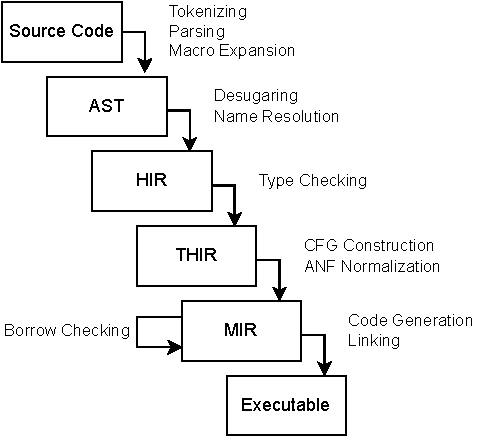
\includegraphics[width=0.7\linewidth]{./rustc-stages.pdf}
	\caption{Diagram providing an overview of the Rustc Compiler Stages}
	\label{fig:rust-stages}
\end{figure}

Figure \ref{fig:rust-stages} shows the the main compiler stages of Rustc and the associated data structure. The first data structure, that is extracted from the source code is the AST (short for abstract syntax tree), which is the result of parsing and expanding macros. 
Based on the AST, the high-level intermediate representation (short HIR) is created by resolving the names and desugaring some language constructs. The HIR contains accurate source labels, which map all nodes in the HIR to their source code locations. 
The HIR is then used as the basis for type checking returning the typed high-level intermediate representation (short THIR), which annotates every node with its type. THIR also lowers some additional constructs like automatic dereferencing and overloading and more. In contrast to the previous representations, "[t]he THIR only represents bodies, i.e. <<executable code>>; this includes function bodies [..]. Consequently, the THIR has no representation for items like \code{struct}s or \code{trait}s." \cite[p. 1]{noauthor_thir_nodate}
THIR will then be used to create the mid-level IR by drastically simplifying the language: The tree structure with complex expression of the THIR is turned in to a control-flow graph (short CFG) with basic blocks containing simple (i.e. non-nested) expressions.

Finally Rustc uses external tools \- like llvm \- to generate executable files and link them.


\chapter{The MiniCorten Language}

Rust's main disadvantage as a target language it its size: There is a lot of syntax and semantics that would need to be accounted. A lot of it even incidental to the verification. To reduce the complexity and amount of work, that needs to be done, we will focus on a subset of Rust described in this section.

The goal is to remove as much incidental complexity as possible without compromising to the central topic of research: How to extend LiquidTypes to mutability under the presence of Rust's ownership model.


\section{Syntax}

\todo{Call it CortenRust (after Weathering Steel)}
This subsection will introduce the syntax of MiniCorten, a language modelled after a simplified version of Rust, with the addition of refinement types.
To simplify the formal definitions and proofs, the language is restricted to ANF\todo{What does the abbrev stand for? XXX Normal Form}, meaning arguments of expressions must be variables. Note that the implementation does not have this restriction.

There are two namespaces for identifiers: $x \in \text{PVar}$ for variables of program variables and $\alpha \in \text{LVar}$ for variable in the refinement predicates. The syntax is defined by the following BNF-Grammar:

\begin{bnfgrammar}
  $program$  ::=
    $func\_decl$ * : function declarations
  ;;
  func\_decl ::=
    $ident$( $param$ * ) -> $ty$ \{ $stmt$ \}
  ;;
  $param$ ::= $x$ \ccolon  $\tau$
  ;;
  $s$: stmt 
  ::=
    $e$                                                   : expression
    | $s_1$; $s_2$                                        : sequence
    | let mut? $x$ = $e$                                  : declaration
    | $x$ = $e$                                           : assignment
    | let $x_v$ = $x_f$($x_1, \dots, x_n$)                : function call
    | while ($x$) \{ $s$ \}                               : while loop
    | if $e_c$ \{ $s_t$ \} else \{ $s_e$ \}               : if statement
    | relax\_ctx!\{ $\varphi$* ; ($x$ \ccolon $\tau$)* \} : context relaxation
  ;;
  $e$                                              : expression 
  ::=
    $ident$                                         : variable reference
    | $lit$                                         : constant
    | $expr$ + $expr$                               : addition
    | * $ident$                                     : dereference
    | \& $ident$                                    : immutable reference
    | \&mut $ident$                                 : mutable reference
    | $expr$ as $ty$                                : type relaxation
  ;;
  $\tau$ : type ::= ty!\{ $logic\_ident$ \ccolon $base\_ty$ \cmid $pred$ \} : refinement type
  ;;
  $\varphi$ : pred ::=
    $ref\_pred$                                     : predicate for a reference type
    | $value\_pred$                                 : predicate for a value type
  ;;
  $ref\_pred$ ::=
    $logic\_ident$ = \& $ident$
    | $ref\_pred$ \cdisj $ref\_pred$         : mutable reference
  ;;
  $value\_pred$ ::=
    $logic\_ident$                : variable
  | $pred$ \&\& $pred$            : conjunction
  | $pred$ \cdisj $pred$          : disjunction
  | ! $pred$                      : negation
  ;;
  $b$: base\_ty ::=
    i32                     : integer
    | unit                  : unit type
    | bool                  : boolean
    | \& $base\_ty$         : immutable reference
    | \&mut $base\_ty$      : mutable reference
  ;;
  $v$: lit ::=
      0,1,...,n             : integer
    | true                  : boolean true
    | false                 : boolean false
    | ()                    : unit value
\end{bnfgrammar}

\section{Semantics}

The semantics are mostly standard. The main difference being that Rust and our simplified language enable most statements to be used in place of an expression. The value is determined by the last statement in the sequence. For example If-Expressions, sequences of statements and function all follow this rule: Their (return) value is determined by the last statement or expression in the sequence.

The semantics loosely based on Jung's MiniRust.

Another difference between Rust and MiniCorten is of course the addition of refinement types.

In terms of the formal description, the rules are similar to Pierce's \cite[p. 166f]{pierce_types_2002-3} "Reference" language. % Also: Semantik von programmiersprachen WhileT p.45
The main difference is, that in Rust, every piece of data has a unique, known owner. This fact makes the concept of locations redundant. Instead we treat $\code{ref}(x)$ as a value itself. The following definitions show the new execution rules.

\begin{definition}[Execution-State]
  The execution state is a partial function from program variables to values: $\sigma : \text{PVar} \rightharpoonup \text{Value}$. 
\end{definition}


\begin{definition}[Evaluation of Expressions: $\bbracket{e} \sigma$ ]
  \begin{align*}
   \bbracket{v} \sigma &= v \\
   \bbracket{x} \sigma &= \sigma(x) \\
   \bbracket{e_1 + e_2} \sigma &= \bbracket{e_1} \sigma + \bbracket{e_2} \sigma \\
   \bbracket{*x} \sigma &= \sigma(y) \qquad \text{if } \sigma(x) = \code{ref}(y) \\
   \bbracket{\code{\&mut } x} \sigma &= \code{ref}(x) \\
   \bbracket{e \code{ as } \tau} \sigma &= \bbracket{e} \\
  \end{align*}
 \end{definition}
 

\begin{definition}[Declaration Environment]
  The environment of function declarations is constant and globally known. It is defined as a partial function $\Sigma : \text{Fn-Name} \rightharpoonup (n, s)$ where $n$ is the number of arguments and $s$ is the body of the function
\end{definition}

\begin{definition}[Small-Step Semantics of MiniCorten: $\tuple{e}{\sigma} \leadsto \tuple{e'}{\sigma'}$]

\begin{gather*}
  \inferrule*[left=SS-Assign]
    {\star}
    {\tuple{x = e }{ \sigma } \leadsto \tuple{\code{unit} }{ \sigma[x \mapsto \bbracket{e}\sigma]}}
  \\
  \inferrule*[left=SS-Decl]
    {\star}
    {\tuple{\code{let } x = e}{\sigma} \leadsto \tuple{unit}{\sigma[ x \mapsto \bbracket{e}\sigma]}}
  \\
  \inferrule*[left=SS-Seq-Inner]
      {\tuple{e_1 }{ \sigma } \leadsto \tuple{e_1' }{ \sigma'}}
      {\tuple{e_1; e_2 }{ \sigma } \leadsto \tuple{e_1'; e_2 }{ \sigma'}}
  \inferrule*[left=SS-Seq-N]
    {\star}
    {\tuple{\code{unit}; e_2 }{ \sigma } \leadsto \tuple{e_2 }{ \sigma'}}
  \\
  \inferrule*[left=SS-IF-T]
    {\bbracket{x} \sigma = \code{true}}
    {\tuple{\code{if } x\ \{ s_t \} \code { else } \{ s_e \} }{\sigma} \leadsto \tuple{s_t}{\sigma}}
  \inferrule*[left=SS-IF-F]
    {\bbracket{x}\sigma = \code{false}}
    {\tuple{\code{if } x\ \{ s_t \} \code { else } \{ s_e \} }{\sigma} \leadsto \tuple{s_e}{\sigma}}
  \\
  \inferrule*[left=SS-While]
    {\star}
    {
      \tuple{ \code{while } e_c\ \{\ s_b \}}{\sigma}
      \leadsto
      \tuple{ \code{if } e_c \{ s_b;  \code{while } e_c \{ s_b \} \} { \code{ else } } \{ \code{unit} \} }{\sigma}
    }
  \\
  \inferrule*[left=SS-Call]
    {\tuple{\Sigma(f)[arg_1 \triangleright x_1, \dots, arg_n \triangleright x_n]}{\sigma} \leadsto \tuple{v_r}{\sigma'} }
    {\tuple{f(x_1, \dots, x_2)}{\sigma} \leadsto \tuple{v_r}{\sigma' \oplus \sigma}}
\end{gather*}

where $$(\sigma' \oplus \sigma)(x) =
  \begin{cases}
    \sigma(x) & \text{if } x = arg_i \\
    \sigma'(x) & \text{if } x \in \text{dom}(\sigma) \cap \text{dom}(\sigma')\\
    \sigma(x) & \text{otherwise }
  \end{cases}$$
\end{definition}

The \textsc{SS-Call} rule does not scope the variables from the callee to the caller. This is actually fine, because by definition variable names are distinct. Therefore only the arguments need to be replaced in the resulting state.

\chapter{The Refinement Type System}


\section{Features}

This subsection will explain some of the key features of the Corten type system.
Corten is directly embedded in Rust using two macros. Firstly the macro \code{ty!} can be used in place of a Rust type and adds a predicate to the Rust type, that any inhabitant of that type must satisfy. For example, the type \code{ty!\{ v : i32 | v >= 0\}} stipulates, that a value of Rust type \code{i32} is positive. The second macro is \code{relax\_ctx!\{ ... \}} which will be explained in subsection \ref{subsec:atomic-updates}.

\subsection{Decidable, Conservative Subtyping}

The idea 

\subsection{Mutable Values}

Corten elected to  \dots
Therefore assigning a new value to a variable will give that variable a new type, but \- crucially \- keep the logic variable in the typing context, which means that types of other variables can still refer to it. Logic variables, that are (no longer) associated with a program variable, are called dangling variables.
That means, that the number of predicates in the context increases with every new value assignment.
In the example, the typing context at the end of the function body contains $v_1$, $v_2$ and their predicates and the association of \code{i} to $v_2$.

There are other approaches for handling changing values in refinement types, which will be described and compared in \ref{subsec:related-work-mutability}.


\begin{listing}[h]
  \begin{minted}[texcomments]{rust}
    fn inc() -> ty!{ v: i32 | v == 3 } {
        let mut i = 2;       // $\{ v_1 : i32 \mid v_1 == 2 \}$
        i = i + 1;           // $\{ v_2 : i32 \mid v_2 == v_1 + 1 \}$
        i
    }
  \end{minted}
  \caption{Example demonstrating why predicates and mutable values may cause problems}
  \label{lst:mutable-values}
\end{listing}

\label{subsec:mutable-references}\subsection{Mutable References}

The key difference to Refinement Type Systems for functional languages to Rust it the pervasive use of mutation. Therefore the most important feature of Corten it the support for mutation and also mutable references.

Corten has two ways of dealing with assignment to mutable references: If the reference destination is known, the destination's type will be updated with the assigned values type (i.e. strong update). If there are multiple possible reference destinations, Corten will require the assigned value to satisfy the predicates of all possible destinations (i.e. weak updates). This is a standard approach (For example \cite{kloos_asynchronous_2015}), but more precise in Rust: The set of possible destinations only grows, when it depends on the execution of an optional control flow path. This means most of the time, strong updates are possible and weak updates are only needed if the reference destination is actually dynamic (i.e. dependent on the execution) \footnote{It would also be possible to encode the path condition in the reference type, but this was decided against for the stated goal of simplicity for the user}

The problem with mutable references is possibility of aliasing. Aliasing is problematic, because it might create interdependencies between the types of different variables: If one variable is changed, it might effect wether another variable is typed correctly. In listing \ref{lst:mutation-strong} the return value \code{a} is effected by changes done to a different variable \code{a}. Conservative approximation requires, that all possible effects must be tracked.

- <dangling>, monotonically increasing $\varphi$

Corten can accurately track references by phrasing them as predicates.
In the example, in \code{b = \&mut a}, \code{\&mut a} will have inferred type \code{\{ r : \&mut | r == \& a \}}, meaning any value of this type can at most refer to to the variable called \code{y}.
When a new value is assigned to \code{*b}, the type system will look at the typing context to find out what \code{b} might refer to. In this case \code{a} is the \textit{only} possible target und we can therefore \textit{update} its type. I.e. in type system, \code{*b = 0} will change the type of \code{a} to \code{\{ s : i32 | s == 0 \}}, but the type of \code{b} stays the same (because it still refers to the same location). We call this kind of assignment a strong assignment, as it can change the type. 

This is sensible, because in Rust's ownership system, \code{a} must be the unique owner of the memory belonging to \code{a}. 
A more involved example is given in the evaluation \ref{subsec:evaluation-complex-mutable-ref}

Note, that the type can only be changed because we know exactly what \code{b} refers to. If there is ambiguity about the destination of a reference, strong updates are no longer possible.



\begin{listing}[h]
  \begin{minted}[texcomments]{rust}
    fn client() -> ty!{ v: i32 | v == 4 } {
        let a = 2;       // $\{ v_1 : i32 \mid v_1 == 2 \}$
        let b = &mut a;  // $\{ v_2 : &i32 \mid v_2 == &a \}$
        *b = 0; // changes a's value and type
        let c = &mut b;
        **c = 4; // changes a's value and type
        a
    }
  \end{minted}
  \caption{Example demonstrating interdependencies between mutable references}
  \label{lst:mutation-strong}
\end{listing}

To support these use cases, Corten also supports weak updates, which can not change types, but allow assigning to ambiguous reference destinations.
The example \ref{lst:mutation-weak} demonstrates how ambiguity about the reference destination may emerge: Depending on the if condition, \code{res} could refer to either \code{y} or \code{z}.
Naturally, we can weaken the reference type to \code{ty!\{ r1 : \&mut i32 | r1 == \&y || r1 == \&z \}}, meaning \code{res} could refer to either \code{y} or \code{z}.
Because the destination is ambiguous, assigning to \code{*res} can not change the type of \code{y} or \code{z}, which is the case if the type of the assigned value is at least as specific as the types of all possible reference destinations.

- importance of tracing return of mutable references



\begin{listing}[h]
  \begin{minted}[texcomments]{rust}
    fn weak_updates(x : ty!{ x1 : i32 }) -> ty!{ v : i32 | v > 2 * x1 + 10 } {
      let mut y = x as ty!{ y1 : i32 | y1 >= x1 };
      let mut z = x + 10 as ty!{ z1 : i32 | z1 >= x1 + 10 };
      let mut res;
      if x > 0 {
        res = &mut y as ty!{ r : &mut | r == &y || r == &z };
                      // branches of if need same type => weaken
      } else {
        res = &mut z as ty!{ r : &mut | r == &y || r == &z };
      }
      *res = x + 11; // res could refer to b or c 
                    // -> assigned value must satisfy both types
      y + z
    }
  \end{minted}
  \caption{Example demonstrating weak updates}
  \label{lst:mutation-weak}
\end{listing}

\label{subsec:path-sensitivify}\subsection{Path Sensitivity}

Firstly, the type system is path sensitive, meaning that the type system is aware of necessary XXX that need to be passed for an expression to be evaluated. For example listing \ref{lst:max-path-sensitive} shows a function computing the maximum of its inputs. In the then branch, $a$ is only a maximum of $a$ and $b$, because the condition $a > b$ implies it. Corten will symbolically evaluate the condition and store it in its typing context.

\begin{listing}[h]
  \begin{minted}{rust}
    fn max(a : ty!{ av: i32 }, b: ty!{ bv: i32 })
        -> ty!{ v: i32 | v >= av && v >= bv} {
        if a > b {
          a as ty!{ x : i32 | x >= av && x >= bv }
        } else {
          b
        }
    }
  \end{minted}
  \caption{Function computing the maximum of its inputs; guaranteeing that the returned value is larger than its inputs}
  \label{lst:max-path-sensitive}
\end{listing}


- inference
- also with mutations


\label{subsec:strong-type-updates}\subsection{Strong Type Updates}

\begin{listing}[h]
  \begin{minted}{rust}
    fn strong_updates(b: ty!{ bv: i32 | bv > 0}) -> ty!{ v: i32 | v > 2} {
        let mut a = 2;
        a = a + b;
        a
    }
  \end{minted}
  \caption{Example of changes to \code{a}'s value effecting its type}
  \label{lst:strong-updates}
\end{listing}



\label{sec:modularity}\subsection{Modularity}

For a verification system to be scalable, it needs to be able modularize a proof. Corten can propagate type information across function calls and by taking advantage of Rust's ownership system, it can do so very accurately. Listing \ref{lst:modular-calls} shows, how an incrementing function \code{inc} can be specified: \code{inc} signature stipulates, that it can be called with any \code{i32} (given the name \code{a1}) and will return a value \code{a2}, which equals \code{a1 + 1}. Only the signature of \code{inc} is necessary for the type checking of \code{client}. 

Notice, that all of the type information about \code{y} is preserved when \code{inc(x)} is called. There are no further annotations needed to type check this program. This is possible, because in safe Rust, any (externally observable) mutation done by a function must be part of the function signature. Corten expands on this, by enabling the user specify exactly how a referenced value is mutated.

\begin{listing}[h]
  \begin{minted}{rust}
    fn inc(a: &mut ty!{ a1: i32 => a2 | a2 == a1 + 1 }) {
      *a = *a + 1;
    }
    fn client(mut x: ty!{ xv: i32 | xv > 2 }) -> ty!{ v: i32 | v > 7 } {
      let mut y = 2;
      inc(&mut x); inc(&mut x);
      inc(&mut y)
      x + y
    }
  \end{minted}
  \caption{Example showing how Corten allows for accurate type checking in the presence of function calls }
  \label{lst:modular-calls}
\end{listing}



\label{subsec:mutual-reference}\subsection{Mutual Reference}

Complex mutation patterns often result in complex interdependencies. We deem it necessary to allow different types to refer to each other.\todo{why?}

\begin{listing}[h]
  \begin{minted}{rust}
      let sum = 0;
      let i = 0;
      
  \end{minted}
  \caption{Function computing the maximum of its inputs; guaranteeing that the returned value is larger than its inputs}
  \label{lst:mutual-reference}
\end{listing}

\label{subsec:atomic-updates}\subsection{Atomic Updates}

- relax ctx
- non-atomic might not be sufficient


\section{Definitions}

\paragraph*{$P$} is the set of program variables used in rust program. Common names $a, b, c$
\paragraph*{$L$} is the set of logic variables used in refinement types. Common names: $\alpha, \beta$

\paragraph*{$\Gamma = (\mu, \Phi)$} is a tuple containing a function $\mu: P \to L$ mapping all program variables to their (current) logic variable and a set of formulas $\Phi$ over $L$. During execution of statements, the set increases monotonically

\paragraph*{$\tau$} is a user defined type $\{ \alpha : b \mid \varphi\}$. Where $\alpha$ is a logic variable from $L$, $b$ is a base type from Rust (like \texttt{i32}) and $\varphi$ is a formula over variables in $L$.

\paragraph*{Abbreviations}
We write:
\begin{itemize}
  \item  $\Gamma, c$ for $(\mu, \Phi \wedge c)$
  \item $\Gamma[a \mapsto \alpha]$ for $(\mu[a \mapsto \alpha], \Phi)$
\end{itemize}


% \section{Expression Typing: $\Gamma \vdash e : \tau \Rightarrow \Gamma'$}

% \begin{gather*}
%   \inferrule*[left=Lit]
%     {l \text{ fresh} \\ \text{base\_ty}(v) = b}
%     {\Gamma \vdash v: \{ l : b \mid l \doteq v\} \Rightarrow \Gamma}
%   %
%   \\
%   \inferrule*[left=Var]
%     {\alpha \text{ fresh} \\ \mu(x) = \beta}
%     {\Gamma = (\mu, \Phi)\vdash x : \{ \alpha : b \mid \beta \doteq \alpha \} \Rightarrow \Gamma}
%   %
%   \\
%   \inferrule*[left=Var-Ref]
%     {\Gamma \vdash y : \tau \\ \Gamma \vdash x : \{ \beta : \&b \mid \beta \doteq \&y \}}
%     {\Gamma \vdash *x : \tau \Rightarrow \Gamma}
%   %
%   \\
%   \inferrule*[left=If]
%     {
%       \Gamma \vdash \mu(x) : \text{bool} \Rightarrow \Gamma
%       \\ \Gamma, \mu(x) \doteq \code{true} \vdash e_t : \tau \Rightarrow \Gamma'
%       \\ \Gamma, \mu(x) \doteq \code{false} \vdash e_e : \tau \Rightarrow \Gamma'
%     }
%     {\Gamma \vdash \text{if } x \text{ then }e_t\text{ else } e_e : \tau \Rightarrow \Gamma'}
%   %
%   \\
%   \inferrule*[left=While]
%     {
%       \Gamma_I, \mu(x) \doteq \code{true} \vdash s \Rightarrow \Gamma_I'
%       \\ \Gamma_I', \mu(x) \doteq \code{true} \preceq \Gamma_I
%     }
%     {\Gamma_I \vdash \texttt{while } x \{ s \} \Rightarrow \Gamma_I,\mu(x) \doteq \code{false}}
%   %
%   \\
%   \inferrule*[left=Seq]
%     {
%       \Gamma \vdash s_1 : \tau_1 \Rightarrow \Gamma'
%       \\ \Gamma' \vdash \bar s : \tau \Rightarrow \Gamma''
%     }
%     {\Gamma \vdash s_1 ; \bar s : \tau \Rightarrow \Gamma''}
%   %
%   \\
%   \inferrule*[left=Add]
%     {
%       \gamma \text{ fresh}
%       \\ \mu(x_1) = \alpha
%       \\ \mu(x_2) = \beta
%     }
%     {\Gamma \vdash x_1 + x_2 : \{ \gamma: b \mid \gamma \doteq \alpha + \beta \} \Rightarrow \Gamma}
%   %
%   \\
%   \inferrule*[left=Decl]
%     {
%       \Gamma \vdash e :  \{ \beta \mid \varphi \} \Rightarrow \Gamma'
%     }
%     {\Gamma \vdash \code{let } x = e : \code{()} \Rightarrow \Gamma'[ x \mapsto \beta], \varphi}
%   %
%   \\
%   \inferrule*[left=Assign]
%     {\Gamma \vdash e : \{ \beta \mid \varphi \} \Rightarrow \Gamma'}
%     {\Gamma \vdash x = e : \code{unit} \Rightarrow \Gamma' [x \mapsto \beta], \varphi}
%   %
%   \\
%   \inferrule*[left=Assign-Strong]
%     {
%       \Gamma \vdash e : \{ \beta \mid \varphi \} \Rightarrow \Gamma'
%       \\ \Gamma \vdash x: \{ \alpha : \& b \mid \alpha \doteq \&y\}
%     }
%     {\Gamma \vdash *x = e : \tau \Rightarrow \Gamma' [y \mapsto \beta], \varphi}
%   %
%   \\
%   \inferrule*[left=Assign-Weak]
%     {
%       \Gamma \vdash e : \tau \Rightarrow \Gamma'
%       \\ \Gamma' \vdash x: \{ \alpha : \& b \mid \alpha \doteq \&y_1 \vee \dots \vee \alpha \doteq \&y_n \} \Rightarrow \Gamma'
%       \\ \Gamma' \vdash \tau \preceq \{ \beta_1 \mid \varphi_1 \}
%       \\ \Gamma'[x \mapsto \beta_1], \varphi_1 \preceq \Gamma'
%       \\\\ \dots
%       \\\\
%       \\ \Gamma' \vdash \tau \preceq \{ \beta_n \mid \varphi_n \}
%       \\ \Gamma'[x \mapsto \beta_n], \varphi_n \preceq \Gamma'
%       }
%     {\Gamma \vdash *x = e : \tau \Rightarrow \Gamma'}
%   %
%   \\
%   \inferrule*[left=Fn-Call]
%     {
%       \text{subst} = ...
%       \\
%       \\ (\mu[subst], \alpha \doteq \mu(a) \wedge \dots \wedge \varphi_{\alpha} \wedge\dots) \preceq (\mu, \Phi)
%       \\ f : (\{ \alpha \mid \varphi_{\alpha} \} \Rightarrow \{ \alpha' \mid \varphi'_{\alpha} \}, \dots) \to \tau
%     }
%     {(\mu, \Phi) \vdash f(a, \dots, \&mut b, \dots) : \tau \Rightarrow (\mu[a \mapsto \alpha', \dots, subst^{-1}], \Phi \wedge \varphi'_{\alpha} \wedge \dots)}
%   %
%   \\
%   \inferrule*[left=Intro-Sub]
%     {
%       \Gamma \vdash e : \tau
%       \\ \Gamma \vdash \tau \preceq \tau'
%     }
%     {\Gamma \vdash e \texttt{ as } \tau': \tau'}
% \end{gather*}

\section{Statement Type Checking $\Gamma \vdash s \Rightarrow \Gamma'$}

\begin{gather*}
  \inferrule*[left=If]
    {
      \Gamma \vdash \mu(x) : \text{bool} \Rightarrow \Gamma
      \\ \Gamma, \mu(x) \doteq \code{true} \vdash s_t \Rightarrow \Gamma'
      \\ \Gamma, \mu(x) \doteq \code{false} \vdash s_e \Rightarrow \Gamma'
    }
    {\Gamma \vdash \text{if } x \text{ then }s_t\text{ else } s_e \Rightarrow \Gamma'}
  %
  \\
  \inferrule*[left=While]
    {
      \Gamma_I, \mu(x) \doteq \code{true} \vdash s \Rightarrow \Gamma_I'
      \\ \Gamma_I', \mu(x) \doteq \code{true} \preceq \Gamma_I
    }
    {\Gamma_I \vdash \texttt{while } x \{ s \} \Rightarrow \Gamma_I,\mu(x) \doteq \code{false}}
  %
  \\
  \inferrule*[left=Seq]
    {
      \Gamma \vdash s_1 \Rightarrow \Gamma'
      \\ \Gamma' \vdash s_2 \Rightarrow \Gamma''
    }
    {\Gamma \vdash s_1 ; s_2 \Rightarrow \Gamma''}
  %
  \\
  \inferrule*[left=Decl]
    {
      \Gamma \vdash e :  \{ \beta \mid \varphi \}
    }
    {\Gamma \vdash \code{let } x = e  \Rightarrow \Gamma'[ x \mapsto \beta], \varphi}
  %
  \\
  \inferrule*[left=Assign]
    {\Gamma \vdash e : \{ \beta \mid \varphi \}}
    {\Gamma \vdash x = e \Rightarrow \Gamma' [x \mapsto \beta], \varphi}
  %
  \\
  \inferrule*[left=Assign-Strong]
    {
      \Gamma \vdash e : \{ \beta \mid \varphi \}
      \\ \Gamma \vdash x: \{ \alpha : \& b \mid \alpha \doteq \&y\}
    }
    {\Gamma \vdash *x = e \Rightarrow \Gamma [y \mapsto \beta], \varphi}
  %
  \\
  \inferrule*[left=Assign-Weak]
    {
      \Gamma \vdash e : \tau
      \\ \Gamma' \vdash x: \{ \alpha : \& b \mid \alpha \doteq \&y_1 \vee \dots \vee \alpha \doteq \&y_n \}
      \\ \Gamma \vdash \tau \preceq \{ \beta_1 \mid \varphi_1 \}
      \\ \Gamma[x \mapsto \beta_1], \varphi_1 \preceq \Gamma
      \\\\ \dots
      \\\\
      \\ \Gamma \vdash \tau \preceq \{ \beta_n \mid \varphi_n \}
      \\ \Gamma[x \mapsto \beta_n], \varphi_n \preceq \Gamma'
      }
    {\Gamma \vdash *x = e \Rightarrow \Gamma'}
  %
  \\
  \inferrule*[left=Fn-Call]
    {
      \text{subst} = ...
      \\
      \\ (\mu[subst], \alpha \doteq \mu(a) \wedge \dots \wedge \varphi_{\alpha} \wedge\dots) \preceq (\mu, \Phi)
      \\ f : (\{ \alpha \mid \varphi_{\alpha} \} \Rightarrow \{ \alpha' \mid \varphi'_{\alpha} \}, \dots) \to \tau
    }
    {(\mu, \Phi) \vdash \code{let res} = f(a, \dots, \code{\&mut} b, \dots) \Rightarrow (\mu[a \mapsto \alpha', \dots, subst^{-1}], \Phi \wedge \varphi'_{\alpha} \wedge \dots)}
\end{gather*}

\section{Expressions Typing: $\Gamma \vdash e : \tau$}

\begin{gather*}
  \inferrule*[left=Lit]
    {l \text{ fresh} \\ \text{base\_ty}(v) = b}
    {\Gamma \vdash v: \{ l : b \mid l \doteq v\} }
  %
  \\
  \inferrule*[left=Var]
    {\alpha \text{ fresh} \\ \mu(x) = \beta}
    {\Gamma = (\mu, \Phi)\vdash x : \{ \alpha : b \mid \beta \doteq \alpha \} }
  %
  \\
  \inferrule*[left=Var-Ref]
    {\Gamma \vdash y : \tau \\ \Gamma \vdash x : \{ \beta : \&b \mid \beta \doteq \&y \}}
    {\Gamma \vdash *x : \tau }
  %
  \\
  \inferrule*[left=Add]
    {
      \gamma \text{ fresh}
      \\ \mu(x_1) = \alpha
      \\ \mu(x_2) = \beta
    }
    {\Gamma \vdash x_1 + x_2 : \{ \gamma: b \mid \gamma \doteq \alpha + \beta \} }
  %
  \\
  \inferrule*[left=Intro-Sub]
    {
      \Gamma \vdash e : \tau
      \\ \Gamma \vdash \tau \preceq \tau'
    }
    {\Gamma \vdash e \texttt{ as } \tau': \tau'}
\end{gather*}


\section{Function Declaration Type Checking}

Without loss of generality, we assume arguments are ordered by their type: First immutable / owner arguments and then mutable arguments.

When handling mutable references in parameters some subtleties need to be considered. The function can change both the referenced \textit{value} as well as the reference \textit{location}. To describe the referenced value is normally done using the $\{ \alpha \mid \alpha \doteq \&b\}$ syntax. The question arises: If $\alpha$ was the logic variable for a parameter, what should be the analog for $b$? In contrast to local variables, there is no variable representing the referenced value for parameters. As seen in section \ref{subsec:mutable-references}, using the dereference operator would come with a lot of complications.
Instead we introduce $arg^i_n$, a special variable denoting the initial abstract value (i.e. stack location), that the mutable reference of argument $n$ points to. $i$ denotes the level of nesting: For the $n$th parameter with the Rust type \code{\&mut \&mut i32} we would generate $arg^1_n$ and $arg^2_n$.

\begin{gather*}
  \inferrule*[left=Fn-Decl]
    { (\{ a_1 \mapsto \alpha_1, b_1 \mapsto \delta_1 \}, \varphi^\alpha_1 \wedge \dots \wedge \delta_1 = arg^1_1 \wedge \varphi^\beta_1 \wedge \dots ) \vdash \bar s \Rightarrow \Gamma'
      \\ \Gamma' \vdash s_{res} : \tau_{res} \Rightarrow \Gamma''
      \\ \Gamma'' \vdash \tau_{res} \preceq \tau
      \\ \Gamma'' \preceq (\{\beta_1 \mapsto \gamma_1\}, \varphi^\gamma_1 )
    }
    {\code{fn } f(a_1 : \{ \alpha_1 \mid \varphi^\alpha_1 \}, \dots, b_1 : \{ \beta_1 \mid \varphi^\beta_1 \Rightarrow \gamma_1 \mid \varphi^\gamma_1\}) \to \tau \{ \bar s; s_{res} \}}
\end{gather*}

\section{Sub-Typing Rules: $\Gamma \vdash \tau \preceq \tau'$}

\[
  \inferrule*[left=$\preceq$-Ty]
    {\Phi \wedge \varphi'[\beta \triangleright \alpha ] \vDash \varphi}
    {\Gamma = (\mu, \Phi) \vdash \{ \alpha \mid \varphi\} \preceq \{ \beta \mid \varphi' \}}
\]

alternative (should be equivalent):

\[
  \inferrule*[left=$\preceq$-Ty-Alt]
    {
      \Gamma[f \mapsto \alpha], \varphi \preceq \Gamma[f \mapsto \beta], \varphi'
      \\ f \text{ fresh}
    }
    {\Gamma \vdash \{ \alpha \mid \varphi\} \preceq \{ \beta \mid \varphi' \}}
\]


\section{Sub-Context Rules: $\Gamma \preceq \Gamma'$}

\[
  \inferrule*[left=$\preceq$-Ctx]
    {
      \Phi'[\mu(\alpha) \triangleright \mu'(\alpha)\ \mid \alpha \in dom(\mu)] \vDash \Phi
      \\ dom(\mu) \subseteq dom(\mu')
    }
    {(\Phi, \mu) \preceq (\Phi', \mu')}
\]

In contrast to other refinement type systems, Corten allows types in the context to refer to one another.
For example a type specifications \code{a : \{ $\alpha$ : i32 | $\alpha$ > $\beta$\}, b:  \{ $\beta$: i32 | $\beta$ != $\alpha$\}} would be valid and result in the context $\Gamma = (\emptyset, \alpha \neq \beta \wedge \beta \geq \alpha)$. In the example, the value $0$ i a valid inhabitant of \code{a}'s type as long as $\code{b} \geq 1$.

This means that types may need to be changed atomically.

\section{Soundness of the Type System}

As usual, we consider the three properties (see Pierce \cite[p. 95, p.167]{pierce_types_2002}) of a type system when assessing the correctness of MiniCorten:

\begin{definition}[State Conformance]
  A state $\sigma$ is conformant with respect to a typing context $\Gamma = (\mu, \varphi)$ (written as $\sigma : \Gamma$), iff:
  $$\vDash \left(\bigwedge_{x \in \text{Var}} \mu(x) \doteq \sigma(x)\right) \to \varphi$$
   I.e. the execution's value assignments imply the type refinements
\end{definition}

\begin{definition}
  Progress:
    If $t$ is closed and well-typed, then $t$ is a value or $t \leadsto t'$, where $t'$ is a value.
\end{definition}

\begin{definition}[Preservation]
  If $\Gamma \vdash e : \tau \Rightarrow \Gamma$ and $e \leadsto e'$, then $\Gamma \vdash e' : \tau \Rightarrow \Gamma$
\end{definition}

The state conformance rule differs from the usual rule in two ways. Firstly we consider the runtime value instead of the runtime type. Secondly there needs to be one set of variable assignments that satisfies all predicates in $\Gamma$.

Because MiniCorten is based on Rust, we will assume, that progress, as well as preservation for the base-types. This includes preservation of type- and ownership-safety. Thus it is sufficient to prove, that assuming these properties hold, preservation of the refinement types is holds.


\begin{lemma}[Conformance of Evaluation]
  If $\sigma : \Gamma$ and $\bbracket{e} \sigma = v$ then $\vDash \varphi \to \bbracket{e} \Gamma$ 
\end{lemma}
% ty!{ == a + b }
% [[a =]]
\begin{proof}
  
\end{proof}


\begin{lemma}[Preservation of State Conformance]
  If $\Gamma \vdash s \Rightarrow \Gamma_2$, $\sigma : \Gamma$ and $\tuple{s}{\sigma} \leadsto \tuple{s_1}{\sigma_1}$, then  $\sigma_1 : \Gamma_1$ and $\Gamma_1 \vdash s_1 \Rightarrow \Gamma_2$ for some $\Gamma_1$
\end{lemma}


\begin{proof} Rule Induction over $\tuple{t}{\sigma} \leadsto \tuple{t'}{\sigma'}$
\begin{itemize}
  \item \textsc{Case SS-Assign}:
    Given $\sigma :: \Gamma$, $\Gamma \vdash x = e \Rightarrow \Gamma_2$
    show $\exists \Gamma_1, \sigma[ x \mapsto \llbracket e \rrbracket \sigma] : \Gamma_1 \wedge \Gamma_1 \vdash \code{unit} \Rightarrow \Gamma_2 $

    Rule inversion over $\Gamma \vdash x = e \Rightarrow \Gamma_2$ gives $\Gamma \vdash e: \{ \alpha : b \mid \alpha \doteq \llbracket e \rrbracket \}$ and $\Gamma_2 = (\Gamma[x \mapsto \alpha], \alpha \doteq \llbracket e \rrbracket)$

    For $\Gamma_1 = \Gamma_2$, $\sigma[x \mapsto \bbracket{e}\sigma ] : (\Gamma[x \mapsto \alpha], \alpha \doteq \llbracket e \rrbracket)$, $\alpha$ is fresh and therefore monotonicity applies.
    
    % Let $v = \llbracket e \rrbracket \sigma$. 
    % For $\Gamma_1 = (\mu[x \mapsto v], \varphi)$

    % $\sigma' = \sigma[x \mapsto v]$. With rule inversion \textsc{Assign}: $e' = \code{unit}$ and post state: $\Gamma'' = \Gamma'[x \mapsto \beta], \varphi$ with $\Gamma \vdash e : \{ \beta \mid \varphi \}$.

    % $e$ is a value, because of the requirement in \textsc{SS-Assign}. By rule inversion \textsc{Lit} over assumption $\Gamma \vdash v: \{ \beta \mid \varphi \} \Rightarrow \Gamma$: $\varphi = (\beta \doteq v)$

    % $\mu'(x) = \beta$, $\sigma'(x) = v$ and induction hypothesis $\sigma : \Gamma$. Since $\mu'(x) \doteq \varphi(x) \to \varphi$ is trivially valid. Monotonicity of State Conformance gives us the goal.

    % Because $e'$ is \code{unit}, the second proof obligation is trivially true, because $\Gamma' = \Gamma''$
  \item \textsc{Case SS-Seq-Inner}:
    Given: $\tuple{c_1}{\sigma} \leadsto \tuple{c_1'}{\sigma'}$, \\
     $\Gamma \vdash c_1 ; c_2 \Rightarrow \Gamma_2$, \\
     $\forall \Gamma_2, \Gamma \vdash c_1 \Rightarrow \Gamma_2 \wedge \sigma : \Gamma \to \exists \Gamma_1, \sigma' : \Gamma_1 \wedge \Gamma_1 \vdash c_1' \Rightarrow \Gamma_2$ \\
    show $\exists \Gamma_1, \sigma' : \Gamma_1 \wedge \Gamma_1 \vdash c_1' ; c_2  \Rightarrow \Gamma_2$.

    Rule inversion over $\Gamma \vdash c_1 ; c_2 \Rightarrow \Gamma_2$ yields $\Gamma \vdash c_1 \Rightarrow \Gamma_1$, $\Gamma_1 \vdash c_2 \Rightarrow \Gamma_2$

    The preconditions for the third induction hypothesis are satisfied for $\Gamma_1$ delivers 
    $\exists \Gamma_1', \sigma' : \Gamma_1' \wedge \Gamma_1' \vdash c_1' \Rightarrow \Gamma_1$

    State conformance $\sigma' : \Gamma_1'$ follows directly from this.

    For $\Gamma_1'$ the preconditions for the \textsc{Seq} rule are satisfied.
  \item \textsc{Case SS-Seq-N}: 
    Given: $\Gamma \vdash \code{unit}; c \Rightarrow \Gamma_2$, $\sigma : \Gamma$
    show $\exists \Gamma_1, \sigma : \Gamma_1 \wedge \Gamma \vdash c \Rightarrow \Gamma_2$.

    Rule inversion over $\Gamma \vdash \code{unit}; c \Rightarrow \Gamma_2$ yields $\Gamma \vdash c \Rightarrow \Gamma_2$.
    Together with the second induction hypothesis this implies the goal.
  \item \textsc{Case SS-Decl}: analogous to \textsc{Case SS-Assign}
  \item \textsc{Case Deref}
    $\sigma(x) = v$, $e' = v$, $\sigma' = \sigma$

    For $\Gamma' = \Gamma$, $\sigma : \Gamma'$ true by assumption

    Show: $\Gamma \vdash v : \tau' \Rightarrow \Gamma$. By rule inversion \textsc{Lit}, $\tau' = \{ l \mid l \doteq v \}$
\end{itemize}
\end{proof}

\begin{lemma}
  State Conformance is monotone\todo{sensible name?}: If $\sigma : \Gamma$, $(\beta = v) \to \varphi$ then
    $\sigma[x \mapsto v] : \Gamma[x \mapsto \beta] \wedge \varphi$
\end{lemma}

\begin{proof}
  $$\vDash \left(\bigwedge_{x \in \text{Var}} \mu(x) \doteq \sigma(x)\right) \to \varphi$$
  ...?
\end{proof}

\label{sec:extensions} \section{Extensions}


To limit the complexity a few features are not defined as part of the Corten or the implementation.
Even though these extensions are not part of the scope of the thesis, these extensions were taken into consideration when designing the type system. To show, that the type system is capable of handling the additional challenges, we will shortly describe how these extensions are planned to be added to the type system.
\todo{move to future work?}

\subsection{Records / \code{struct}s}

Firstly, a key part of realistic programs are data structures that comprise multiple basic data types. In Rust these are called \code{struct}s and work similar to records or product types in functional languages. 

Once again, we can take advantage of Rust ownership system: Any part of a struct (even nested fields) can only belong to one variable. This means, that the proposed system for handling mutable references extends seamlessly to structs: 
The variable mapping in $\Gamma$ is generalized: $\mu : \text{Path} \to \text{LVar}$. The relevant typing rules will work without major changes:

\begin{gather*}
  \inferrule*[left=Var]
    {\mu(p.x.y.z) = \alpha}
    {\Gamma \vdash p.x.y.z : \{ \beta \mid \beta \doteq \alpha \} \Rightarrow \Gamma}
    \\
  \inferrule*[left=Assign-Strong]
    {\Gamma \vdash e : \tau}
    {\Gamma \vdash p.x.y.z = e : \code{unit} \Rightarrow \Gamma[p.x.z.y \mapsto \tau]}
\end{gather*}

\subsection{Algebraic Data Types}

With records added, the only thing missing for support of algebraic data types are sum types.
Sum types allow the programmer to express, that an inhabitant of a type may be one variant of a set of multiple fixed options: For example the result of a fallible computation may either be \code{Ok(V)} meaning a successful computation with the result \code{V} or a failure \code{Err(E)} with a description of the error \code{E}.
In rust these sum types are called \code{enum}s.

Sum types influence the type system in two key ways: 

Firstly, the specification of its values. Suppose a programmer would like an authentication function signature to state, that the function returns an \code{Err} code "403" if the password was incorrect. This requires the type language to assert what variant is expected as well as access to its fields (if the variant is known).

Secondly, path sensitivity needs to be extended to cover \code{match} expressions (called \code{case} is most functional programming languages). \code{match} expression allow the programmer to branch depending on the variant of a value.

\subsection{Inference}

While the current implementation is able to type expressions without explicit type annotations, solving a set of type constraints is not implemented. 
Rondon et al. \cite{rondon_liquid_2008} describe a mechanism to infer complex refined types by combining known predicates from the context. This approach should be adaptable to Corten to reduce the amount of needed type annotations even further.


\subsection{Predicate Generics}

Vazou et al. \cite{vazou_abstract_2013} found, that the expressiveness of refinement types can still be expanded without leaving a decidable fragment by adding uninterpreted functions to the logic. In the type system, these uninterpreted functions represent "abstract predicates". At the definition site, abstract predicates can not be inspected and restricted, but the caller can instantiate then with a concrete predicate.



\chapter{Implementation: CortenC}

The type system described in the previous chapter was implemented to test the practical feasibility of our approach.
There are a few differences and details between the type system described above and the implementation CortenC (short for Corten Checker) that will be highlighted in this chapter.

In contrast to the MiniCorten and the described type system, CortenC uses actual Rust as its target language. In addition to MiniCorten's features, CortenC also covers expressions with side-effects, non-ANF expressions, statements as well as basic inference.
These features do not change the expressiveness of the type system, but make it a lot more practical.

\paragraph{Target Selection}
% Target selection: HIR / MIR?
The architecture of the rustc compiler makes it possible to implement a refinement type system quite cleanly: Rustc's plugin system allows CortenC to access rustc's intermediate representations and also emit diagnostics with source locations. Since the diagnostics from CortenC use the same interface as Rust's diagnostics, other tools like IDEs can handle them without any adaptation.

CortenC uses the HIR. It is a good candidate for extensions to the type system, because it contains source labels, allowing accurate problem reporting to the user. Secondly, in HIR all names are resolved making and types can be queried for HIR nodes, which means the Rustc plugin can reuse a lot of work done in the Rustc Compiler. Thirdly, non-executable segments of the program, like type declarations, are represented in the HIR.

Using MIR is also a sensible option: The MIR is a drastically simplified representation of just the executable segments of the program as a CFG with non-nested expressions. Because of the simplicity, it would be appealing to use the MIR as the basis for the implementation. 
An additional advantage of MIR could be, that ownership analysis is done on MIR, which would allow the refinement type system to use that information. Surprisingly, we did not encounter any situation, where ownership information is necessary for typing refined types.

Ultimately, it was decided against using the MIR for the following reasons:
Firstly a concern for the quality of diagnostics: The MIR code is quite distant from the user-provided code. For example, when trying to explain a error when typing a while-loop, the implementation may need to reconstruct the original source code structure from the CFG, which could be inaccurate and error-prone. 
In addition, source locations may be less accurate or unavailable. 
Finally the MIR does not contain type declarations, which could make it hard to extend the implementation for algebraic data type or predicate generics (see section \ref{sec:extensions})

\paragraph{Language Embedding}
CortenC exposes a minimal interface to the programmer: The interface consists of two macros:
\code{ty!\{ ... \}} which allows the programmer to specify a refined type for a rust base type and
\code{relax\_ctx!\{ ... \}} to allow the programmer to relax the typing context (mostly used for introducing a loop-invariant). 

Listing \ref{lst:macro-definition} shows how the \code{ty!} macros is defined: Most important are the first two macro forms, which handle immutable types like \code{ty!\{ v : i32 | v > 0\}} and mutable parameter types like \code{ty!\{ v1: i32 | v1 > 0 => v2 | v2 < 0\}}. 
There are additional short forms of these macro calls, which where cut from the listing for brevity. Both macro calls are translated into the type alias \code{Refinement} (\code{MutRefinement} respectively). For the examples above, it would be \code{Refinement<i32, "v", "v > 0">} and \code{MutRefinement<i32, "v1", "v1 > 0", "v2", "v2 > 0">} respectively. These type aliases are quite useful for CortenC: They ensure, that CortenC keeps compatibility with Rust. I.e. a program with CortenC type annotations can be compiled in normal Rust without problems and the type aliases also simplify the implementation of CortenC, because the refined type can be extracted directly from the Rust type alias. Consequently, CortenC does not need to perform name resolution, even for external function declarations.

Note that, because the \code{ty!} macro takes the place of a Rust type, normal IDE features, like "Goto Type Definition" still work on the base types without any adaptation.

\begin{listing}[h]
  \begin{minted}[autogobble]{rust}
  pub type Refinement<
    T,                      // Rust type
    const B: &'static str,  // Logic Variable
    const R: &'static str   // Predicate
  > = T;

  pub type MutRefinement<
      T,                      // Rust type
      const B1: &'static str, // Logic Variable Before
      const R1: &'static str, // Predicate Before
      const B2: &'static str, // Logic Variable After
      const R2: &'static str, // Predicate After
  > = T;

  #[macro_export]
  macro_rules! ty {
    ($i:ident : $base_ty:ty | $pred:expr) => {
        $crate::Refinement< $base_ty, {stringify! { $i }}, {stringify! { $pred }}>
    };
    ($i:ident : $base_ty:ty | $pred:expr => $i2: ident | $pred2:expr) => {
        $crate::MutRefinement< $base_ty, {stringify! { $i }}, {stringify! { $pred }}, {stringify! { $i2 }}, {stringify! { $pred2 }}>
    };
    // -- snip --
  }
  \end{minted}
  \caption{Definition of CortenC's macros}
  \label{lst:macro-definition}
\end{listing}

For the second macro \code{relax\_ctx!} takes the place of a statement. 
It is translated to a function call, that can then be used to reconstruct the described context.

\paragraph{Architecture}
CortenC follows the structure implied by the type system: All concepts and type checking rules have a correspondence in CortenC:
\code{RContext} is the representation of $\Gamma$ in CortenC, with the main difference being, that predicates stay associated with a logic variable (and potentially a program variable). The purpose being, that in the future, CortenC could create better error messages, by associating "blame" to a type checking failure: If the predicate of a logic variable is part of the reason why a subtyping check fails, it would be useful to convey that information to the user. 
\code{RefinementType} is the representation of $\tau$ in CortenC.

CortenC registers a callback in Rustc to run after HIR construction. The callback calls \code{type\_check\_function} for each function in the HIR, which either returns \code{Result::Ok} indicating, that the function type checks or \code{Result::Err} if type checking failed. In that case, the callback will emit a diagnostic to rustc to inform the user about the refinement type error.
Listing \ref{lst:architecture-cortenc} shows the core functions signatures involved in type checking. \code{type\_check\_function} corresponds to the \textsc{Fn-Decl} rule by constructing the initial context and delegating checking of the body to \code{type\_expr}. 
Since Rust expressions can contain statements, \code{type\_expr} will use \code{transition\_stmt} to type check these statements before returning the final type context.
Both \code{type\_expr} and \code{transition\_stmt} carry a collection of parameters, that contain the Rust type checking data (The global type context \code{TyCtxt} and the local type context \code{TypeckResults}), the refinement type context \code{RContext}, a handle to the SMT solver \code{SmtSolver} and a way to generate fresh logic variable names \code{Fresh}.

These function utilize \code{require\_is\_sub\_context} and \code{require\_is\_subtype\_of} to dispatch the actual SMT solver requests. These functions are also responsible for encoding the predicates and substituting variable names where necessary. 
The following paragraph will give an example for how these SMT solver requests look like.

\begin{listing}[h]
  \begin{minted}[autogobble, texcomments]{rust}
  fn type_check_function(
    function: &hir::Item,
    tcx: &TyCtxt,
  ) -> Result<RefinementType> { .. }

  fn transition_stmt(
    stmts: &a [hir::Stmt],
    tcx: & TyCtxt,
    ctx: & RContext,
    local_ctx: & TypeckResults,
    solver: &mut SmtSolver,
    fresh: &mut Fresh,
  ) -> Result<RContext> { .. }

  fn type_expr(
    expr: &a Expr,
    tcx: & TyCtxt,
    ctx: & RContext,
    local_ctx: & TypeckResults,
    solver: &mut SmtSolver,
    fresh: &mut Fresh,
  ) -> Result<(RefinementType, RContext)> { .. }

  fn require_is_sub_context(
    super_ctx: &RContext,
    sub_ctx: &RContext,
    tcx: &TyCtxt,
    solver: &mut SmtSolver,
  ) -> anyhow::Result<()> { .. }

  fn require_is_subtype_of(
      sub_ty: &RefinementType,
      super_ty: &RefinementType,
      ctx: &RContext,
      tcx: &TyCtxt,
      solver: &mut SmtSolver,
  ) -> anyhow::Result<()> { .. }
  \end{minted}
  \caption{Overview of the central function CortenC is built from. (Lifetimes were removed for clarity)}
  \label{lst:architecture-cortenc}
\end{listing}

\paragraph{Simple Example}

\begin{listing}[h]
  \begin{minted}[autogobble, texcomments]{rust}
  fn inc(a : ty!{ n : i32 | n > 0}) -> ty!{v : i32 | v > 1} {
    let b = 1;
    a + b
  }
  \end{minted}
  \caption{Simple Example Program used for demonstrating the operation of CortenC}
  \label{lst:simple-example-cortenc}
\end{listing}

Consider the example program \ref{lst:simple-example-conrtenc}, which returns the increment of the argument.
Rustc will call the CortenC callback with the item \code{fn inc} once the HIR construction is completed. Next, the callback calls \code{type\_check\_function} where the initial context $\Gamma = ( a \mapsto n, \left\{ n > 0\right\})$ is constructed and calls \code{type\_expr} with the the function body expression. Base the function body is a sequence \code{transition\_stmt} is called for all expect the last expression in the sequence. \code{let b = 1} updates the context to $\Gamma_1 = ( a \mapsto n, b \mapsto v_1, \left\{ n > 0, v_1 = 1\right\})$ ($v_1$ is a name generated by \code{Fresh}). 
Finally \code{type\_expr} types the expression \code{a + b} according to the typing rules described above resulting in the type $\left\{ v_2 : i32 \mid v_2 = n + v_1\right\}$.
This type is then returned as the overall type of the body expression to \code{type\_check\_function}, which has the responsibility of checking that in the context $\Gamma_1$, the actual return type is a subtype of the specified type in the signature. 
Thusly \code{require\_is\_subtype\_of} is called with the two types and subsequently dispatches the SMT shown in listing \ref{smt-sample-output}. 
Because the SMT call returned \code{unsat}, the subtype relation is valid and the function type checking was successful.


\begin{listing}[h]
  \begin{minted}[autogobble]{lisp}
    (declare-datatypes () ((Unit unit)))

    ; <Context>
      ; decl for <fud.rs>:79:73: 79:74 (#0) local b
      (declare-const _0 Int)
      
      ; decl for <fud.rs>:79:9: 79:10 (#0) local a
      (declare-const n Int)
      
      ; predicate for _0: local b
      ;     ty!{ _0 : i32 | _0 == 1 }
      (assert
          (= |_0| 1)
      )
      
      ; predicate for n: local a
      ;     ty!{ n : i32 | n > 0 }
      (assert
          (> |n| 0)
      )
    ; </Context>

    (declare-const _1 Int)
    (assert
        (= (+ |n| |_0|) |_1|)
    )
    
    (assert
        (not (> |_1| 1))
    )
    
    ; checking: ty!{ _1 : i32 | n + _0 == _1 } ≼  ty!{ v : i32 | v > 1 }
    (check-sat)
    
    ; done checking is_subtype_of! is sat: false
  \end{minted}
  \caption{SMT Requests dispatched by CortenC for checking that the returned type matches the specified type}
  \label{lst:smt-sample-output}
\end{listing}

% -[x] Type Aliases
% -[x] working without special compiler
% -[x] compiler plugin
% -[x] IDE
% -[x] HIR
% -[x] Location data (spans)
% -[x] signatures
% -[x] Additional features
%   -[x] basic inference
%   -[x] no ANF
%   -[x] side-effectful expressions
% - [x] z3 example prompt

\chapter{Evaluation}

In this chapter Corten will be tested on a selection of examples to test the practicality.

\section{Maximum using Path Conditions}

The first example will show how a the \code{max} function can be implemented and fully verified in CortenC. The mathematical maximum is defined as $r = max(a, b) iff r \geq a \wedge r \geq b \wedge (r == a \vee r == b)$. Listing \ref{lst:eval-max} shows how this can be expressed in CortenC.


\begin{listing}[h]
  \begin{minted}[autogobble, texcomments]{rust}
  fn max(a: ty!{ a: i32 }, b: ty!{ b: i32}) 
    -> ty!{ v: i32 | v >= a && v >= b && (v == a || v == b) } {
    if a > b {
        a as ty!{ x: i32 | x >= a && x >= b && (x == a || x == b) }
    } else {
        b
    }
  }
  \end{minted}
  \caption{Example demonstrating a fully specified \code{max} function using Corten's path sensitivity}
  \label{lst:eval-max}
\end{listing}

Of course an incorrect implementation will produce a type judgement error. If, for example, the else branch returned \code{a} instead of \code{b}, the system would return the error shown in listing \ref{lst:eval-max-error}. The exact location of where the error occurred is also the current implementation does not expose this data yet.

\begin{listing}[h]
  \begin{minted}[autogobble]{text}
  Subtyping judgement failed: 
  ty!{ _1 : i32 | true && _1 == a } is not a sub_ty of 
  ty!{ v : i32 | v >= a && v >= b && (v == a || v == b) } 

  in ctx RContext {
    // formulas
    // types
    local a : ty!{ a : i32 | true }
    local b : ty!{ b : i32 | true }
  }
  \end{minted}
  \caption{Example of an error message created by CortenC}
  \label{lst:eval-max-error}
\end{listing}

Path sensitivity is not limited to the return value: Effect on the type context can also be path sensitive as demonstrated by listing \ref{lst:eval-clamp}, which implements a clamping function. The function \code{clamp} ensures, that the reference passed to it will be at most \code{max} or stay the same. \code{client} uses \code{clamp} and can use the facts from \code{clamp}'s mutation specification when proving its own return type specification.

Note, that when typing \code{client}, CortenC needs to match \code{\&mut x} with \code{a} and thusly \code{x} with \code{s} to correctly handle the effects of calling \code{clamp}. Because of this reason, function calls require all arguments to be variables or reference to variables. This is not a restriction of the type system, but a simplification for the implementation.

\begin{listing}[h]
  \begin{minted}[autogobble, texcomments]{rust}
  fn clamp(
      a: &mut ty!{ a1: i32 | true => s | (s <= max) && (s == a1 || s == max) }, 
      max: ty!{ max: i32 }
  ) -> ty!{ v:  () } {
      if *a > max {
          *a = max as ty!{ r | (r <= max) && (r == a1 || r == max) }; ()
      } else {};
      ()
  }

  fn client() -> ty!{ v : i32 | v == 42 } {
      let mut x = 1337; let max = 42;
      clamp(&mut x, max);
      x
  }
  \end{minted}
  \caption{Example demonstrating optional mutation of an external location}
  \label{lst:eval-clamp}
\end{listing}

\section{Recursion: Fibonacci-Numbers}

Thanks to Corten's modular approach, handling recursive functions is strait forward in CortenC. Listing \ref{lst:eval-fib} demonstrates this by implementing a function, that returns the $n$th fibonacci number $F_n$ and asserting that $F_n \geq n^2$. Because $n$ is arbitrary, this is proves that the fibonacci sequence grows faster than the $n^2$.


\begin{listing}[h]
  \begin{minted}[autogobble, texcomments]{rust}
    fn fib(n: ty!{ nv: i32 | nv >= 0}) -> ty!{ v: i32 | v >= nv * nv } {
      if n >= 2 {
          let n1 = n - 1; let n2 = n - 2;

          let f1 = fib(n1); let f2 = fib(n2);
          (f1 + f2) as ty!{ r : i32 | r >= nv * nv }
      } else {
          1
      }
    }
  \end{minted}
  \caption{Example demonstrating recursive function calls by proving a divergence property of the fibonacci sequence}
  \label{lst:eval-fib}
\end{listing}


\section{Loop Invariants: Proof of the Gauss Summation Formula}

The next example demonstrates, that CortenC can also verify loop invariants. Listing \ref{lst:gauss} shows a function, that calculates the sum $\sum_{i = 1}^N i$ by repeatedly increment a variable by $i$. 
Of course there exists a closed formula computing the same result: $n \cdot (n + 1) \over 2$, which is given as the specification. CortenC will therefore proof, that the closed form return the same result compared to the iterative summation.

This example is quite challenging, because of interdependencies between \code{i} and \code{sum} in the invariant as well as the old value of \code{i} and old values of \code{sum} in the loop body. 

To proof, that the invariant holds after each loop body execution, we need the exact information, that \code{i} was incremented by one and \code{sum} by \code{i} as well as the knowledge, that \code{i} and \code{sum} satisfied the predicates. Corten solves this problem by treating predicates as immutable and retaining "dangling" predicates (i.e. no longer associated with a program variable).

The second challenge is establishing the loop invariant in the first place: Relaxing the type of \code{i} from $= 0$ to $\leq nv$ is only valid, because we know relaxing the type of \code{sum} from $= 0$ to $ 2 * sv == iv * (iv + 1)$ is valid if $iv = 0$ and vice versa: To update the type of \code{sum} first, we need the knowledge, that $iv = 0$, but once we relax the type of \code{i}, \code{i} gets a new logic variable, which is distinct from the logic variable used in the type of \code{sum}. Thus the loop invariant needs to be established atomically.

For this purpose, CortenC provides the \code{relax\_ctx!} macro, that allows the programmer to change the type of multiple variables at a time, as long as the previous state \textit{as a whole} implies the newly chosen predicates.

\begin{listing}[h]
  \begin{minted}[autogobble, texcomments]{rust}
  fn gauss(n: ty!{ nv : i32 | nv > 0 }) 
  -> ty!{ v : i32 | 2 * v == nv * (nv + 1) } {
    let mut i = 0;
    let mut sum = 0;
    
    // Loop Invariant:
    relax_ctx!{
        n |-> nv | nv > 0,
        i |-> iv | iv <= nv,
        sum |-> sv | 2 * sv == iv * (iv + 1)
    }
    while i < n {
        i = (i + 1);
        sum = (sum + i);
    }
    sum
  }
  \end{minted}
  \caption{Example loops with complex loop invariants and value updates effecting the invariant}
  \label{lst:gauss}
\end{listing}

\label{subsec:evaluation-complex-mutable-ref}\section{Complex Mutable References}



\section{Rephrasing built-ins in terms of Refinement Types}

The following example demonstrates, that Corten naturally extends to unusual edge cases and still allows easy verification based on them.
Rust has built-in functions for aborting execution \- called \code{panic} \- and a function for conditionally aborting execution \- called \code{assert}. Listing \ref{lst:eval-builtins} shows a reimplementation of these functions with full refined type specifications. 
\code{panic} asserts that after a call to it, \code{false} is valid. This naturally follows from inverting the path condition after exiting the loop. 
\code{assert} also uses the path condition to assert the correctness of \code{cond} and uses panic for the else case. The return type of \code{assert} can use the logic variable \code{c} from the input directly as the predicate, that is satisfied after the execution.
The \code{client} just needs to make sure, that the proof of \code{c} is stored in the context by storing the value in the variable \code{\_witness}: If the returned value is discarded, it will not be stored in the context and therefore will not be available when proving the return value specification.


\begin{listing}[h]
  \begin{minted}[autogobble, texcomments]{rust}
  fn panic() -> ty!{ v : () | false } {
      while(true) { () }
  }

  fn assert(cond: ty!{ c : bool }) -> ty!{ v: () | c } {
      if cond {
          () as ty!{ v: () | c }
      } else {
          panic()
      }
  }

  fn client(a : ty!{ av: i32 }) -> ty!{ v: i32 | v > 0 } {
      let arg = a > 0;
      let _witness = assert(arg);
      a
  }
  \end{minted}
  \caption{Example showing how \code{panic} and \code{assert} can be naturally specified and verified in CortenC}
  \label{lst:eval-builtins}
\end{listing}


\section{Extendability with Other tools}

- Corten: only safe
- Expend Corten by using external tools to verify unsafe
- use assert to tell Corten what to assume and external tool what to verify

\chapter{Related Work}

There currently does not exist an implementation of refinement types for Rust.

Relevant papers originate from two lines of work. Firstly additions to refinement types for mutability, asynchronous execution etc. and secondly other verification frameworks for Rust.

For example, Lanzinger \cite{lanzinger_property_2021} successfully adapted refinement types to Java, which allows the user to check, that property types described by java annotations hold true throughout the program. At this point in time, specification and verification is limited to immutable (\code{final}) data.

Kloos et al. \cite{kloos_asynchronous_2015} extended refinement types to mutable and asynchronous programs. The paper explores how changes to possibly aliased memory cells can be tracked throughout a OCaml program. For that purpose the types are extended by a set of requirements on memory objects, which track distinctness and refined types of these memory cells. In contrast to OCaml, Rust already guarantees that mutable memory is not aliased and in particular \textit{all mutable memory locations must be accessible by a variable name in the current context}, which offers substantial advantages in terms of simplicity to specification and verification of Rust programs.

Refinement types are also used in other applications. For example Graf et al. \cite{graf_lower_2020} use refinement types to check the exhaustiveness of pattern matching rules over complex (G)ADT types in Haskell. To check the exhaustiveness of patterns in Liquid Rust with ADTs may require similar approaches.

In terms of alternative verification approaches, Prusti\cite{astrauskas_leveraging_2019} is notable, because of their work on formalizing the full Rust semantics, including \code{unsafe}. Prusti is a heavy-weight functional verification framework for Rust; based on separation logic.

Alternative verification approaches also exists: For example RustHorn\cite{matsushita_rusthorn_2020} employs constrained horn clauses based verification to Rust. Particularity relevant for this thesis is the novel formalization for mutable references used in the paper. The authors stipulate that mutable references should be specified by a pre- and post-state from before a reference is borrowed to after it is returned.

The notion of Abstract Refinement Types that this thesis is based on is defined by Vazou et al. \cite{vazou_abstract_2013}. The basic idea is to allow the programmer to "refine" language types with predicates from a decidable logic. The type system has a notion of subtyping for refined types, where one type is a subtype of another if one predicate implies the other.

\label{subsec:related-work-mutability} \subsection{Alternative Approaches for Handling Mutability}

Of course the design space permits choosing other tradeoffs. For example, Rondon et al. \cite{rondon_low-level_2010} chooses 
  - only interdependence in single record using fold mechanism
  - 

this is not the only way to deal with mutability: 

\section{Comparison to Flux}

\chapter{Conclusion \& Future Work}

\printbibliography

\end{document}